\documentclass[a4paper,11pt]{jvetdoc}

\usepackage{geometry}[2010/02/12]

\usepackage{hyperref}
\hypersetup{colorlinks=true,
            linkcolor=black,      % color of internal links (change box color with linkbordercolor)
            citecolor=black,      % color of links to bibliography
            filecolor=black,      % color of file links
            urlcolor=blue}
\usepackage{color,soul}

\usepackage[position=bottom]{subfig}
\captionsetup[subfloat]{position=top}
\usepackage{multirow}
\usepackage{dcolumn}
\newcolumntype{.}{D{.}{.}{-1}}
\usepackage{colortbl}
\usepackage{makecell}
\usepackage{longtable}
\usepackage{array}
\usepackage{algorithm2e}
\usepackage{amsmath}

\urlstyle{same}

% code highlighting
\usepackage{minted,xcolor}
\definecolor{bggray}{gray}{0.95}
\setminted{
bgcolor=bggray,
xleftmargin=3ex,
breaklines=true,
fontsize=\footnotesize}


\usepackage[strings]{underscore}
\usepackage{csquotes}
\MakeOuterQuote{"}
\EnableQuotes

\newcommand\None{}
\newcommand\NotSet{}
\makeatletter
\newcommand{\Option}[1]{\ifx\optOption\@empty\gdef\optOption{#1}\else\g@addto@macro\optOption{ \\ #1}\fi}
\newcommand{\ShortOption}[1]{\ifx\optShortOption\@empty\gdef\optShortOption{#1}\else\g@addto@macro\optShortOption{ \\ #1}\fi}
\newcommand{\Default}[1]{\ifx\optDefault\@empty\gdef\optDefault{#1}\else\g@addto@macro\optDefault{ \\ #1}\fi}
\newcommand{\clearOptions}{\gdef\optOption{}\gdef\optShortOption{}\gdef\optDefault{}}
\makeatother
\newenvironment{OptionTable}[1]{%
	\footnotesize
	\def\arraystretch{1.8}
	\clearOptions
	\begin{longtable}{l<{\makecell[tl]{\optOption}}%
	                  >{\texttt\bgroup}l<{\makecell[tl]{\optShortOption}\egroup}%
	                  c<{\makecell[tc]{\optDefault}}%
	                  >{\def\arraystretch{1.0}}p{0.5\textwidth}<{\clearOptions}}
	\caption{#1} \\
	\hspace*{12em}&&\hspace*{8em}&\kill
	\hline
	 \thead{Option} &
	 \egroup\thead{Shorthand}\bgroup &
	 \thead{Default} &
	 \thead{Description} \\
	\hline
	\endfirsthead
	\caption[]{#1 (Continued)} \\
	\hspace*{12em}&&\hspace*{8em}&\kill
	\hline
	 \thead{Option} &
	 \egroup\thead{Shorthand}\bgroup &
	 \thead{Default} &
	 \thead{Description} \\
	\hline
	\endhead
	 \multicolumn{4}{r}{Continued...}\\
	 \hline
	\endfoot
	 \hline
	\endlastfoot
}{%
	\hline
	\end{longtable}
}

\newenvironment{OptionTableNoShorthand}[2]{%
	\scriptsize
	\def\arraystretch{1.8}
	\clearOptions
	\begin{longtable}{l<{\makecell[tl]{\optOption}}%
	                  c<{\makecell[tc]{\optDefault}}%
	                  >{\def\arraystretch{1.0}}p{0.5\textwidth}<{\clearOptions}}
	\caption{#1} \label{#2} \\
	\hspace*{12em}&\hspace*{8em}&\kill
	\hline
	 \thead{Option} &
	 \thead{Default} &
	 \thead{Description} \\
	\hline
	\endfirsthead
	\caption[]{#1 (Continued)} \\
	\hspace*{12em}&\hspace*{8em}&\kill
	\hline
	 \thead{Option} &
	 \thead{Default} &
	 \thead{Description} \\
	\hline
	\endhead
	 \multicolumn{3}{r}{Continued...}\\
	 \hline
	\endfoot
	 \hline
	\endlastfoot
}{%
	\hline
	\end{longtable}
}

\newenvironment{SEIListTable}[1]{%
	\scriptsize
	\def\arraystretch{1.8}
	\clearOptions
	\begin{longtable}{c<{\makecell[tl]{\optOption}}%
	                  l<{\makecell[tc]{\optDefault}}%
	                  >{\def\arraystretch{1.0}}p{0.3\textwidth}<{\clearOptions}}
	\caption{#1} \\
	\hspace*{12em}&\hspace*{8em}&\kill
	\hline
	 \thead{SEI Number} &
	 \thead{SEI Name} &
	 \thead{Table number of encoder controls, if available} \\
	\hline
	\endfirsthead
	\caption[]{#1 (Continued)} \\
	\hspace*{12em}&\hspace*{8em}&\kill
	\hline
	 \thead{SEI Number} &
	 \thead{SEI Name} &
	 \thead{Table number of encoder controls, if available} \\
	\hline
	\endhead
	 \multicolumn{3}{r}{Continued...}\\
	 \hline
	\endfoot
	 \hline
	\endlastfoot
}{%
	\hline
	\end{longtable}
}

\newenvironment{MacroTable}[1]{%
	\scriptsize
	\def\arraystretch{1.3}
	\clearOptions
	\begin{longtable}{lcp{0.5\textwidth}}
	 \caption{#1} \\
	%\hspace*{12em}&&\hspace*{8em}&\kill
	 \hline
	  \thead{Option} &
	  \thead{Default} &
	  \thead{Description} \\
	 \hline
	\endfirsthead
	 \caption[]{#1 (Continued)} \\
	 \hline
	  \thead{Option} &
	  \thead{Default} &
	  \thead{Description} \\
	 \hline
	\endhead
	 \multicolumn{3}{r}{Continued...}\\
	 \hline
	\endfoot
	 \hline
	\endlastfoot
}{%
	\end{longtable}
}

\title{VTM Software Manual}
\author{%
	Frank Bossen
	\email{frank@bossentech.com}
	\and
	David Flynn
	\email{dflynn@blackberry.com}
	\and
	Xiang Li
	\email{xlxiangli@tencent.com}
	\and
	Karl Sharman
	\email{karl.sharman@eu.sony.com}
	\and
	Karsten S\"uhring
	\email{karsten.suehring@hhi.fraunhofer.de}
}

\jvetmeeting{}
\jvetdocnum{Software Manual}
\jvetdocstatus{Software AHG working document}
\jvetdocpurpose{Information}
\jvetdocsource{AHG chairs}

\begin{document}
\maketitle
\begin{abstract}
This document is a user manual describing usage of the VTM reference software
for the VVC project. It applies to version 5.2 of the software.
\end{abstract}

\tableofcontents
\listoftables


\section{General Information}
Reference software is being made available to provide a reference
implementation of the HEVC standard being developed by the Joint 
Video Experts Team (JVET) regrouping experts from
ITU-T SG 16 and ISO/IEC SC29 WG11. One of the main goals of the
reference software is to provide a basis upon which to conduct
experiments in order to determine which coding tools provide desired
coding performance. It is not meant to be a particularly efficient
implementation of anything, and one may notice its apparent
unsuitability for a particular use. It should not be construed to be a
reflection of how complex a production-quality implementation of a
future VVC standard would be.

This document aims to provide guidance on the usage of the reference
software. It is widely suspected to be incomplete and suggestions for
improvements are welcome. Such suggestions and general inquiries may be
sent to the general JVET email reflector on
\url{https://lists.rwth-aachen.de/postorius/lists/jvet.lists.rwth-aachen.de/} 
(registration required).

\subsection*{Bug reporting}
Bugs should be reported on the issue tracker set up at:

\url{https://jvet.hhi.fraunhofer.de/trac/vvc/}

\section{Installation and compilation}
The software may be retrieved from the GitLab server located at:

\url{https://vcgit.hhi.fraunhofer.de/jvet/VVCSoftware_VTM}

Table~\ref{tab:project-files} lists the compiler environments and versions 
for which building the software is tested.

Note that the software makes use of C++11 language features, which may not
be available in older compilers.

\begin{table}[ht]
\caption{Supported compilers}
\label{tab:project-files}
\centering
\begin{tabular}{ll}
\hline
 \thead{Compiler environment} &
 \thead{Versions} \\
\hline
MS Visual Studio  & 2015 and 2017 \\
GCC               & 5.4 and 7.3 \\
Xcode/clang       & latest \\
\hline
\end{tabular}
\end{table}

By default the software is built as 64-bit binaries to be used on a 64-bit OS. 
This allows the software to use more than 2GB of RAM.

The software uses CMake to create platform-specific build files. 

\subsection {Build instructions for plain CMake (suggested)}

\textbf{Note:} A working CMake installation is required for building the software.

CMake generates configuration files for the compiler environment/development
environment on each platform. The following is a list of examples for Windows
(MS Visual Studio), macOS (Xcode) and Linux (make).

Open a command prompt on your system and change into the root directory
of this project.

Create a build directory in the root directory:
\begin{minted}{bash}
mkdir build 
\end{minted}
Use one of the following CMake commands, based on your platform. Feel free to change the 
commands to satisfy your needs.

\textbf{Windows Visual Studio 2015 64 Bit:}
\begin{minted}{bash}
cd build
cmake .. -G "Visual Studio 14 2015 Win64"
\end{minted}
Then open the generated solution file in MS Visual Studio.

\textbf{macOS Xcode:}
\begin{minted}{bash}
cd build
cmake .. -G "Xcode"
\end{minted}
Then open the generated work space in Xcode.

\textbf{Linux}

For generating Linux Release Makefile:
\begin{minted}{bash}
cd build
cmake .. -DCMAKE_BUILD_TYPE=Release
\end{minted}
For generating Linux Debug Makefile:
\begin{minted}{bash}
cd build
cmake .. -DCMAKE_BUILD_TYPE=Debug
\end{minted}
Then type
\begin{minted}{bash}
make -j
\end{minted}
to build the software.

For more details, refer to the CMake documentation: \url{https://cmake.org/cmake/help/latest/}

\subsection {Build instructions for make}

\textbf{Note:}
The build instructions in this section require the make tool and Python
to be installed, which are part of usual Linux and macOS environments. 
See section \ref{windowsinstall} for installation instruction for Python 
and GnuWin32 on Windows.

Open a command prompt on your system and change into the root directory
of this project.

To use the default system compiler simply call:
\begin{minted}{bash}
make all
\end{minted}
For MSYS2 and MinGW:
Open an MSYS MinGW 64-Bit terminal and change into the root directory
of this project.

Call:
\begin{minted}{bash}
make all toolset=gcc
\end{minted}

\subsection{Tool Installation on Windows}
\label{windowsinstall}

Download CMake: \url{http://www.cmake.org/} and install it.

Python and GnuWin32 are not mandatory, but they simplify the build process for the user.

\begin{table}[ht]
\footnotesize
\centering
\begin{tabular}{ll}
\hline
Python     &    \url{https://www.python.org/downloads/release/python-371/} \\
GnuWin32   &    \url{https://sourceforge.net/projects/getgnuwin32/files/getgnuwin32/0.6.30/GetGnuWin32-0.6.3.exe/download} \\
\hline
\end{tabular}
\end{table}

To use MinGW, install MSYS2:
\url{http://repo.msys2.org/distrib/msys2-x86_64-latest.exe}

Installation instructions:
\url{https://www.msys2.org/}

Install the needed toolchains:
\begin{minted}{bash}
pacman -S --needed base-devel mingw-w64-i686-toolchain mingw-w64-x86_64-toolchain git subversion mingw-w64-i686-cmake mingw-w64-x86_64-cmake
\end{minted}

%%%%
%%%%
%%%%
\section{Using the encoder}

\begin{minted}{bash}
TAppEncoder 	[--help] [-c config.cfg] [--parameter=value]
\end{minted}

\begin{table}[ht]
\footnotesize
\centering
\begin{tabular}{lp{0.5\textwidth}}
\hline
 \thead{Option} &
 \thead{Description} \\
\hline
\texttt{--help} & Prints parameter usage. \\
\texttt{-c} & Defines configuration file to use.  Multiple configuration files
     may be used with repeated --c options. \\
\texttt{--}\emph{parameter}\texttt{=}\emph{value}
    & Assigns value to a given parameter as further described below.
      Some parameters are also supported by shorthand
      "--\em{opt}~\emph{value}". These are shown in brackets after the parameter
      name in the tables of this document\\
\hline
\end{tabular}
\end{table}

Sample configuration files are provided in the cfg/ folder.
Parameters are defined by the last value encountered on the command line.
Therefore if a setting is set via a configuration file, and then a subsequent
command line parameter changes that same setting, the command line parameter
value will be used.

\subsection{GOP structure table}
\label{sec:gop-structure}
Defines the cyclic GOP structure that will be used repeatedly
throughout the sequence. The table should contain GOPSize lines,
named Frame1, Frame2, etc. The frames are listed in decoding
order, so Frame1 is the first frame in decoding order, Frame2 is
the second and so on. Among other things, the table specifies all
reference pictures kept by the decoder for each frame. This
includes pictures that are used for reference for the current
picture as well as pictures that will be used for reference in
the future. The encoder will not automatically calculate which
pictures have to be kept for future references, they must
be specified. Note that some specified reference frames for
pictures encoded in the very first GOP after an IDR frame might
not be available. This is handled automatically by the encoder,
so the reference pictures can be given in the GOP structure table
as if there were infinitely many identical GOPs before the
current one. Each line in the table contains the parameters used
for the corresponding frame, separated by whitespace:

\begin{itemize}
\item[]\textbf{Type}: Slice type, can be either I, P or B.

\item[]\textbf{POC}: Display order of the frame within a GOP, ranging
from 1 to GOPSize.

\item[]\textbf{QPOffset}: QP offset is added to the QP parameter to set
the final QP value to use for this frame.

\item[]\textbf{QPOffsetModelOff}: Offset parameter to a linear model to adjust final QP based on QP + QPoffset.

\item[]\textbf{QPOffsetModelScale}: Scale parameter to a linear model to adjust final QP based on QP + QPoffset.

\item[]\textbf{SliceCbQPOffset}: The slice-level Cb QP offset.

\item[]\textbf{SliceCrQPOffset}: The slice-level Cr QP offset.

\item[]\textbf{QPFactor}: Weight used during rate distortion
optimization. Higher values mean lower quality and less bits. Typical
range is between
0.3 and 1.

\item[]\textbf{tcOffsetDiv2}: In-loop deblocking filter parameter tcOffsetDiv2 
is added to the base parameter LoopFilterTcOffset_div2 to set the final tc_offset_div2 
parameter for this picture signalled in the slice segment header. The final 
value of tc_offset_div2 shall be an integer number in the range $-6..6$.

\item[]\textbf{betaOffsetDiv2}: In-loop deblocking filter parameter betaOffsetDiv2 
is added to the base parameter LoopFilterBetaOffset_div2 to set the final beta_offset_div2 
parameter for this picture signalled in the slice segment header. The final 
value of beta_offset_div2 shall be an integer number in the range $-6..6$.

\item[]\textbf{temporal_id}: Temporal layer of the frame. A frame cannot
predict from a frame with a higher temporal id. If a frame with higher
temporal IDs is listed among a frame's reference pictures, it is
not used, but is kept for possible use in future frames.

\item[]\textbf{num_ref_pics_active_L0}: Number of reference pictures in lists L0
that are used during coding.

\item[]\textbf{num_ref_pics_L0}: Size of reference picture list L0.
This includes pictures that are used for reference for the
current picture as well as pictures that will be used for reference in
the future.

\item[]\textbf{reference_pictures_L0}: A space-separated list of
num_ref_pics integers, specifying the POC of the reference pictures
kept, relative the POC of the current frame. The picture list shall be
ordered as their intendend order in the L0.
Note that any pictures not supplied in this list and in the list of L1 will be discarded and
therefore not available as reference pictures later.

\item[]\textbf{num_ref_pics_active_L1}: Number of reference pictures in lists L1
that are used during coding.

\item[]\textbf{num_ref_pics_L1}: Size of reference picture list L1.
This includes pictures that are used for reference for the
current picture as well as pictures that will be used for reference in
the future.

\item[]\textbf{reference_pictures_L1}: A space-separated list of
num_ref_pics integers, specifying the POC of the reference pictures
kept, relative the POC of the current frame. The picture list shall be
ordered as their intendend order in the L1.
Note that any pictures not supplied in this list and in the list of L0 will be discarded and
therefore not available as reference pictures later.

For example, consider the coding structure of Figure~\ref{fig:gop-example}.
This coding structure is of size 4. The pictures are listed in decoding
order. Frame1 shall therefore describe picture with $\textrm{POC}=4$. It
references picture 0, and therefore has 4 as a reference picture.
Similarly, Frame2 has a POC of 2, and since it references pictures 0 and
4, its reference pictures are listed as \verb|2 -2|. Frame3 is a special
case: even though it only references pictures with POC 0 and 2, it also
needs to include the picture with POC 4, which must be kept in order to
be used as a reference picture in the future. Note that picture with POC 4 can be
included in the L0 or L1. The reference picture list for Frame3 therefore becomes \verb|1 -1 -3|. 
Frame4 has a POC of 3 and its list of reference pictures is \verb|1 -1|.
\end{itemize}

\begin{figure}[h]
\caption{A GOP structure}
\label{fig:gop-example}
\centering
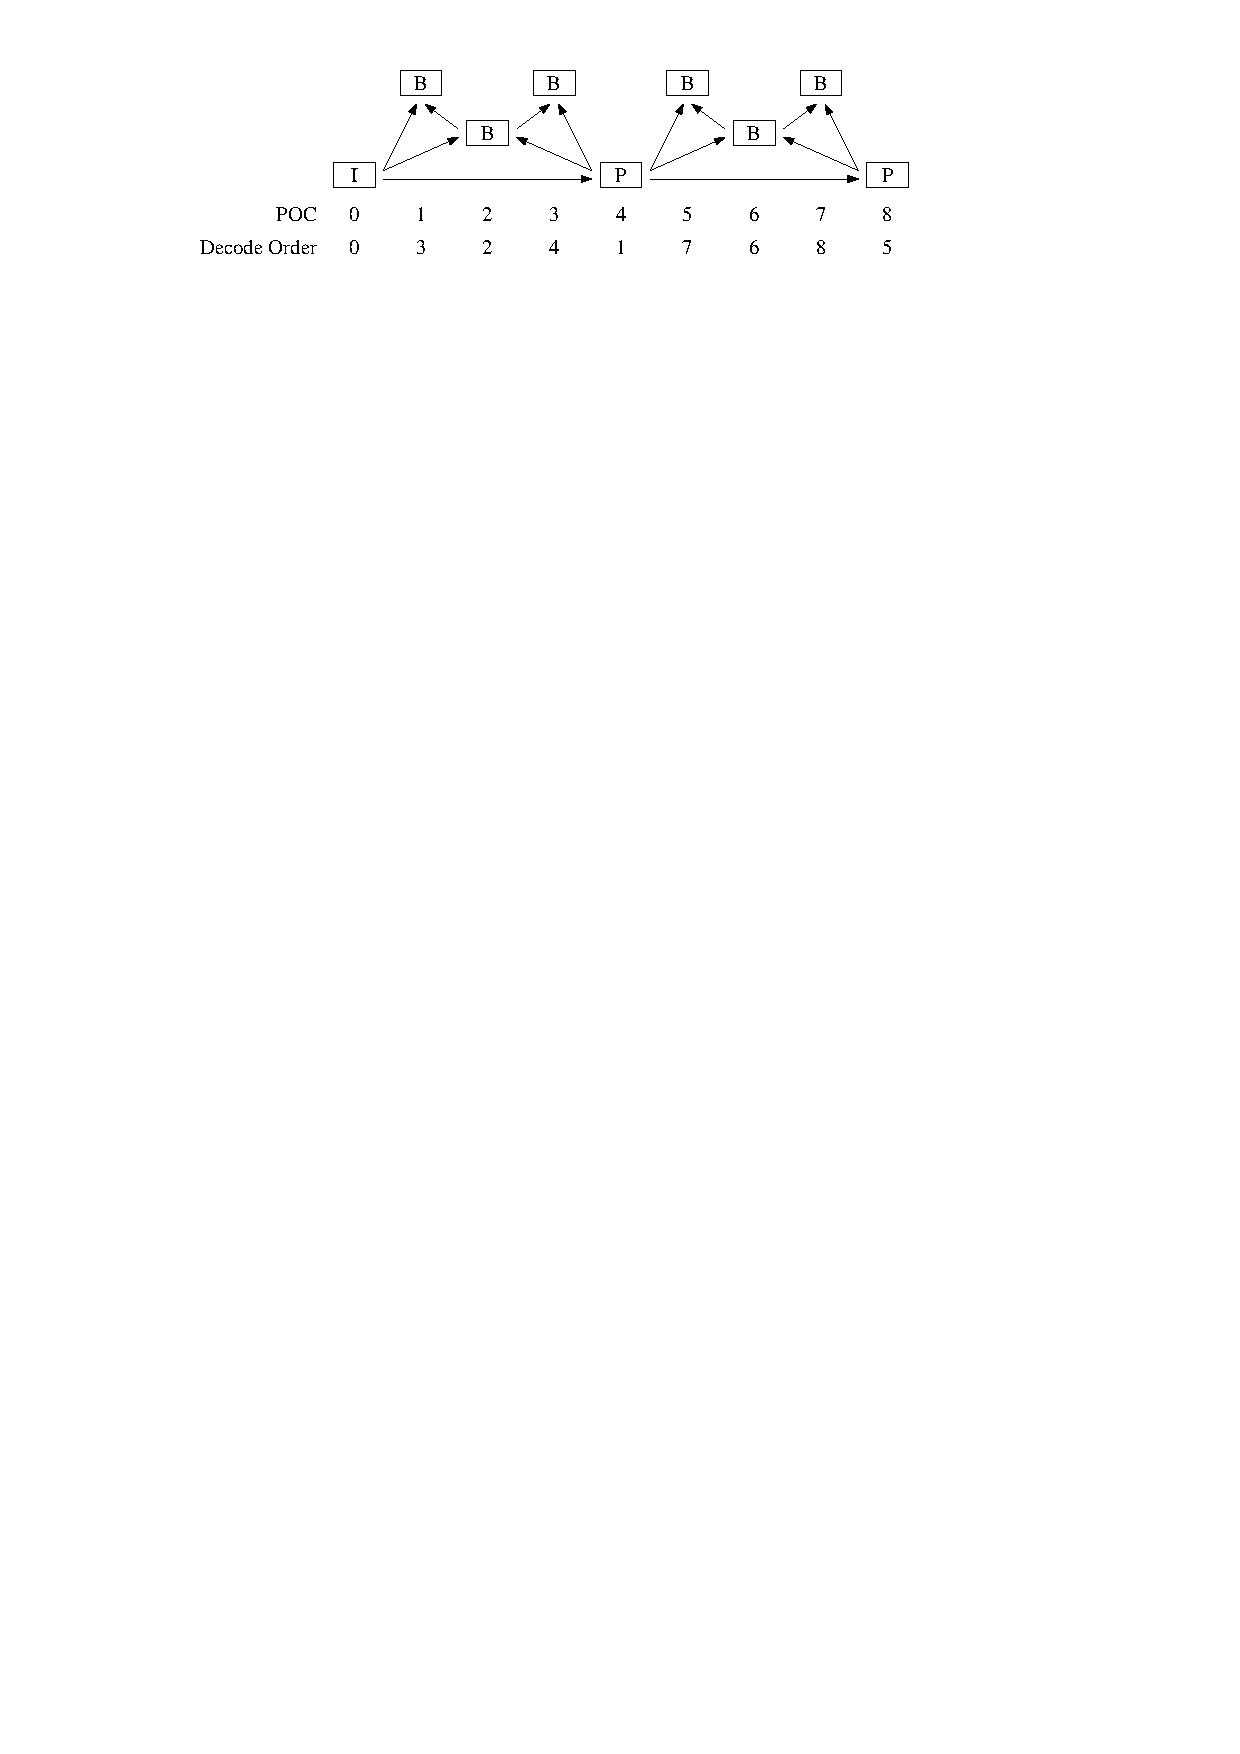
\includegraphics[width=0.7\textwidth]{figures/gop-structure-example}
\end{figure}

In order to specify this to the encoder, the parameters in
Table~\ref{tab:gop-example} could be used.

\begin{table}[ht]
\footnotesize
\caption{GOP structure example}
\label{tab:gop-example}
\centering
\begin{tabular}{lrrrr}
\hline
 \thead{} &
 \thead{Frame1} &
 \thead{Frame2} &
 \thead{Frame3} &
 \thead{Frame4} \\
\hline
Type                   &   P  &    B   &         B   &       B \\
POC                    &   4  &    2   &         1   &       3 \\
QPOffset               &   1  &    2   &         3   &       3 \\
QPOffsetModelOff       & 0.0  &  0.0   &       0.0   &     0.0 \\
QPOffsetModelScale     & 0.0  &  0.0   &       0.0   &     0.0 \\
SliceCbQPOffset        &   0  &    0   &         0   &       0 \\
SliceCrQPOffset        &   0  &    0   &         0   &       0 \\
QPfactor               & 0.5  &  0.5   &       0.5   &     0.5 \\
tcOffsetDiv2           &   0  &    1   &         2   &       2 \\  
betaOffsetDiv2         &   0  &    0   &         0   &       0 \\
temporal_id            &   0  &    1   &         2   &       2 \\
num_ref_pics_active_L0 &   1  &    1   &         1   &       1 \\
num_ref_pics_L0        &   1  &    1   &         1   &       1 \\
reference_pictures_L0  &   4  &    2   &         1   &       1 \\
num_ref_pics_active_L1 &   0  &    1   &         1   &       1 \\
num_ref_pics_L1        &   0  &    1   &         2   &       1 \\
reference_pictures_L1  &      & $-$2   & $-$1 $-$3   &    $-$1 \\
\hline
\end{tabular}
\end{table}

Here, the frames used for prediction have been given higher
quality by assigning a lower QP offset. Also, the non-reference
frames have been marked as belonging to a higher temporal layer,
to make it possible to decode only every other frame. Note: each
line should contain information for one frame, so this
configuration would be specified as:

\begin{verbatim}
Frame1: P 4 1 0 0 0.5 0 0 0 1 1  4 1 1  4
Frame2: B 2 2 0 0 0.5 1 0 1 1 1  2 1 1 -2
Frame3: B 1 3 0 0 0.5 2 0 2 1 1  1 1 2 -1 -3
Frame4: B 3 3 0 0 0.5 2 0 2 1 1  1 1 1 -1
\end{verbatim}




%%%%
%%%%
%%%%
\newgeometry{tmargin=1.6cm,lmargin=1cm,rmargin=1cm,bmargin=1in,nohead}
\subsection{Encoder parameters}

%%
%% File, I/O and source parameters
%%
Shorthand alternatives for the parameter that can be used on the command line are shown in brackets after the parameter name.

\begin{OptionTableNoShorthand}{File, I/O and source parameters.}{tab:fileIO}
\Option{InputFile (-i)} &
%\ShortOption{-i} &
\Default{\NotSet} &
Specifies the input video file.

Video data must be in a raw 4:2:0, or 4:2:2 planar format, 4:4:4 planar format (Y$'$CbCr, RGB or GBR), or in a raw 4:0:0 format. 

Note: When the bit depth of samples is larger than 8, each sample is encoded in
2 bytes (little endian, LSB-justified).
\\

\Option{BitstreamFile (-b)} &
%\ShortOption{-b} &
\Default{\NotSet} &
Specifies the output coded bit stream file.
\\

\Option{ReconFile (-o)} &
%\ShortOption{-o} &
\Default{\NotSet} &
Specifies the output locally reconstructed video file.
\\

\Option{SourceWidth (-wdt)}%
\Option{SourceHeight (-hgt)} &
%\ShortOption{-wdt}%
%\ShortOption{-hgt} &
\Default{0}%
\Default{0} &
Specifies the width and height of the input video in luma samples.
\\

\Option{InputBitDepth}
 &
%\ShortOption{\None} &
\Default{8} &
Specifies the bit depth of the input video.
\\

\Option{MSBExtendedBitDepth} &
%\ShortOption{\None} &
\Default{0} &
Extends the input video by adding MSBs of value 0. When 0, no extension is applied and the InputBitDepth is used.

The MSBExtendedBitDepth becomes the effective file InputBitDepth for subsequent processing.
\\

\Option{InternalBitDepth} &
%\ShortOption{\None} &
\Default{0} &
Specifies the bit depth used for coding. When 0, the setting defaults to the
value of the MSBExtendedBitDepth.

If the input video is a different bit depth to InternalBitDepth, it is
automatically converted by:
\begin{displaymath}
\left\lfloor
 \frac{\mathrm{Pel} * 2^{\mathrm{InternalBitDepth}}}{
     2^{\mathrm{MSBExtendedBitDepth}}}
\right\rfloor
\end{displaymath}

Note: The effect of this option is as if the input video is externally
converted to the MSBExtendedBitDepth and then to the InternalBitDepth
and then coded with this value as InputBitDepth. The codec has no
notion of different bit depths.
\\

\Option{OutputBitDepth} &
%\ShortOption{\None} &
\Default{0} &
Specifies the bit depth of the output locally reconstructed video file.
When 0, the setting defaults to the value of InternalBitDepth.
Note: This option has no effect on the decoding process.
\\

\Option{InputBitDepthC}%
\Option{MSBExtendedBitDepthC}%
\Option{InternalBitDepthC}%
\Option{OutputBitDepthC} &
%\ShortOption{\None} &
\Default{0}%
\Default{0}%
\Default{0}%
\Default{0} &
Specifies the various bit-depths for chroma components.  These only need
to be specified if non-equal luma and chroma bit-depth processing is
required. When 0, the setting defaults to the corresponding non-Chroma value.
\\

\Option{InputColourSpaceConvert} &
%\ShortOption{\None} &
\Default{\NotSet} &
The colour space conversion to apply to input video. Permitted values are:
\par
\begin{tabular}{lp{0.3\textwidth}}
  UNCHANGED & No colour space conversion is applied \\
  YCbCrToYCrCb & Swap the second and third components \\
  YCbCrtoYYY & Set the second and third components to the values in the first \\
  RGBtoGBR & Reorder the three components \\
\end{tabular}
\par
If no value is specified, no colour space conversion is applied. The list may eventually also include RGB to YCbCr or YCgCo conversions.
\\

\Option{SNRInternalColourSpace} &
%\ShortOption{\None} &
\Default{false} &
When this is set true, then no colour space conversion is applied prior to PSNR calculation, otherwise the inverse of InputColourSpaceConvert is applied.
\\

\Option{OutputInternalColourSpace} &
%\ShortOption{\None} &
\Default{false} &
When this is set true, then no colour space conversion is applied to the reconstructed video, otherwise the inverse of InputColourSpaceConvert is applied.
\\

\Option{InputChromaFormat} &
%\ShortOption{\None} &
\Default{420} &
Specifies the chroma format used in the input file. Permitted values (depending on the profile) are 400, 420, 422 or 444.
\\

\Option{ChromaFormatIDC (-cf)} &
%\ShortOption{-cf} &
\Default{0} &
Specifies the chroma format to use for processing. Permitted values (depending on the profile) are 400, 420, 422 or 444; the value of 0 indicates that the value of InputChromaFormat should be used instead.
\\

\Option{MSEBasedSequencePSNR} &
%\ShortOption{\None} &
\Default{false} &
When 0, the PSNR output is a linear average of the frame PSNRs; when 1, additional PSNRs are output which are formed from the average MSE of all the frames. The latter is useful when coding near-losslessly, where occasional frames become lossless.
\\

\Option{PrintFrameMSE} &
%\ShortOption{\None} &
\Default{false} &
When 1, the Mean Square Error (MSE) values of each frame will also be output alongside the default PSNR values.
\\

\Option{PrintSequenceMSE} &
%\ShortOption{\None} &
\Default{false} &
When 1, the Mean Square Error (MSE) values of the entire sequence will also be output alongside the default PSNR values.
\\

\Option{SummaryOutFilename} &
%\ShortOption{\None} &
\Default{false} &
Filename to use for producing summary output file. If empty, do not produce a file.
\\

\Option{SummaryPicFilenameBase} &
%\ShortOption{\None} &
\Default{false} &
Base filename to use for producing summary picture output files. The actual filenames used will have I.txt, P.txt and B.txt appended. If empty, do not produce a file.
\\

\Option{SummaryVerboseness} &
%\ShortOption{\None} &
\Default{false} &
Specifies the level of the verboseness of the text output.
\\

\Option{CabacZeroWordPaddingEnabled} &
%\ShortOption{\None} &
\Default{false} &
When 1, CABAC zero word padding will be enabled. This is currently not the default value for the setting.
\\

\Option{ConformanceWindowMode} &
%\ShortOption{\None} &
\Default{0} &
Specifies how the parameters related to the conformance window are interpreted (cropping/padding).
The following modes are available:
\par
\begin{tabular}{cp{0.43\textwidth}}
0 & No cropping / padding \\
1 & Automatic padding to the next minimum CU size \\
2 & Padding according to parameters HorizontalPadding and VerticalPadding \\
3 & Cropping according to parameters ConfWinLeft, ConfWinRight, ConfWinTop and ConfWinBottom \\
\end{tabular}
\\

\Option{HorizontalPadding (-pdx)}%
\Option{VerticalPadding (-pdy)} &
%\ShortOption{-pdx}%
%\ShortOption{-pdy} &
\Default{0} &
Specifies the horizontal and vertical padding to be applied to the input
video in luma samples when ConformanceWindowMode is 2.  Must be a multiple of
the chroma resolution (e.g. a multiple of two for 4:2:0).
\\

\Option{ConfWinLeft}%
\Option{ConfWinRight}%
\Option{ConfWinTop}%
\Option{ConfWinBottom} &
%\ShortOption{\None} &
\Default{0} &
Specifies the horizontal and vertical cropping to be applied to the
input video in luma samples when ConformanceWindowMode is 3. 
Must be a multiple of the chroma resolution (e.g. a multiple of
two for 4:2:0).
\\

\Option{FrameRate (-fr)} &
%\ShortOption{-fr} &
\Default{0} &
Specifies the frame rate of the input video.

Note: This option only affects the reported bit rates.
\\

\Option{FrameSkip (-fs)} &
%\ShortOption{-fs} &
\Default{0} &
Specifies a number of frames to skip at beginning of input video file.
\\

\Option{FramesToBeEncoded (-f)} &
%\ShortOption{-f} &
\Default{0} &
Specifies the number of frames to be encoded (see note regarding TemporalSubsampleRatio). When 0, all frames are coded.
\\

\Option{TemporalSubsampleRatio (-ts)} &
%\ShortOption{-fs} &
\Default{1} &
Temporally subsamples the input video sequence. A value of $N$ will skip $(N-1)$ frames of input video after each coded input video frame. Note the FramesToBeEncoded does not account for the temporal skipping of frames, which will reduce the number of frames encoded accordingly. The reported bit rates will be reduced and VUI information is scaled so as to present the video at the correct speed. The minimum and default value is 1.
\\

\Option{FieldCoding} &
%\ShortOption{\None} &
\Default{false} &
When 1, indicates that field-based coding is to be applied.
\\

\Option{TopFieldFirst (-Tff)} &
%\ShortOption{\None} &
\Default{0} &
Indicates the order of the fields packed into the input frame. When 1, the top field is temporally first.
\\

\Option{ClipInputVideoToRec709Range} &
%\ShortOption{\None} &
\Default{0} &
If 1 then clip input video to the Rec. 709 Range on loading when InternalBitDepth is less than MSBExtendedBitDepth.
\\

\Option{ClipOutputVideoToRec709Range} &
%\ShortOption{\None} &
\Default{0} &
If 1 then clip output video to the Rec. 709 Range on saving when OutputBitDepth is less than InternalBitDepth.
\\

\Option{EfficientFieldIRAPEnabled} &
%\ShortOption{\None} &
\Default{1} &
Enable to code fields in a specific, potentially more efficient, order.
\\

\Option{HarmonizeGopFirstFieldCoupleEnabled} &
%\ShortOption{\None} &
\Default{1} &
Enables harmonization of Gop first field couple.
\\

\Option{AccessUnitDelimiter} &
%\ShortOption{\None} &
\Default{0} &
Add Access Unit Delimiter NAL units between all Access Units.
\\

\end{OptionTableNoShorthand}

%%
%% profile, level and conformance options
%%
\begin{OptionTableNoShorthand}{Profile and level parameters}{tab:profile}
\Option{Profile} &
%\ShortOption{\None} &
\Default{none} &
Specifies the profile to which the encoded bitstream complies.

Valid HEVC Ver. 1 values are: none, main, main10, main-still-picture

Valid HEVC Ver. 2 (RExt) values are: main-RExt, high-throughput-RExt,
monochrome, monochrome12, monochrome16, main12, main_422_10,
main_422_12, main_444, main_444_10, main_444_12, main_444_16,
main_intra, main_10_intra, main_12_intra, main_422_10_intra, main_422_12_intra,
main_444_intra, main_444_10_intra, main_444_12_intra, main_444_16_intra.

When main-RExt is specified, the constraint flags are either manually specified, or calculated via the other supplied settings.

Compatibility flags are automatically determined according to the profile.
NB: There is currently only limited validation that the encoder configuration complies with the profile, level and tier constraints.
\\

\Option{Level} &
%\ShortOption{\None} &
\Default{none} &
Specifies the level to which the encoded bitstream complies.
Valid values are: none, 1, 2, 2.1, 3, 3.1, 4, 4.1, 5, 5.1, 5.2, 6, 6.1, 6.2, 8.5

NB: There is currently only limited validation that the encoder configuration complies with the profile, level and tier constraints.
\\

\Option{Tier} &
%\ShortOption{\None} &
\Default{main} &
Specifies the level tier to which the encoded bitsream complies.
Valid values are: main, high.

NB: There is currently only limited validation that the encoder configuration complies with the profile, level and tier constraints.
\\

\Option{SubProfile} &
%\ShortOption{\None} &
\Default{0} &
Indicates interoperability metadata registered as specified by X Recommendation ITU-T T.35.
\\

\Option{EnableDecodingParameterSet} &
%\ShortOption{\None} &
\Default{false} &
Enables writing of a decoding parameter set. If disabled, no parameter set will be written and the specical reserved ID zero will be used in the SPS indicating no constraint.
\\

\Option{MaxBitDepthConstraint} &
%\ShortOption{\None} &
\Default{0} &
For --profile=main-RExt, specifies the value to use to derive the general_max_bit_depth constraint flags for RExt profiles; when 0, use $\max(InternalBitDepth, InternalBitDepthC)$
\\

\Option{MaxChromaFormatConstraint} &
%\ShortOption{\None} &
\Default{0} &
For --profile=main-RExt, specifies the chroma-format to use for the general profile constraints for RExt profiles; when 0, use the value of ChromaFormatIDC.
\\

\Option{IntraConstraintFlag} &
%\ShortOption{\None} &
\Default{false} &
For --profile=main-RExt, specifies the value of general_intra_constraint_flag to use for RExt profiles.
\\

\Option{OnePictureOnlyConstraintFlag} &
%\ShortOption{\None} &
\Default{false} &
For --profile=main-RExt, specifies the value of general_one_picture_only_constraint_flag to use for RExt profiles.
\\

\Option{LowerBitRateConstraintFlag} &
%\ShortOption{\None} &
\Default{true} &
Specifies the value of general_lower_bit_constraint_flag to use for RExt profiles.
\\

\Option{ProgressiveSource} &
%\ShortOption{\None} &
\Default{false} &
Specifies the value of general_progressive_source_flag
\\

\Option{InterlacedSource} &
%\ShortOption{\None} &
\Default{false} &
Specifies the value of general_interlaced_source_flag 
\\

\Option{NonPackedSource} &
%\ShortOption{\None} &
\Default{false} &
Specifies the value of general_non_packed_constraint_flag
\\

\Option{FrameOnly} &
%\ShortOption{\None} &
\Default{false} &
Specifies the value of general_frame_only_constraint_flag
\\

\end{OptionTableNoShorthand}


%%
%% Unit definition parameters
%%

\begin{OptionTableNoShorthand}{Unit definition parameters}{tab:unit}
\Option{MaxCUWidth} &
%\ShortOption{\None} &
\Default{64} &
Defines the maximum CU width.
\\

\Option{MaxCUHeight} &
%\ShortOption{\None} &
\Default{64} &
Defines the maximum CU height.
\\

\Option{MaxCUSize (-s)} &
%\ShortOption{\None} &
\Default{64} &
Defines the maximum CU size.
\\

\Option{MaxPartitionDepth (-h)} &
%\ShortOption{-h} &
\Default{4} &
Defines the depth of the CU tree.
\\

\Option{QuadtreeTULog2MaxSize} &
%\ShortOption{\None} &
\Default{6 \\ ($= \mathrm{log}_2(64)$)} &
Defines the Maximum TU size in logarithm base 2.
\\

\Option{QuadtreeTULog2MinSize} &
%\ShortOption{\None} &
\Default{2 \\ ($= \mathrm{log}_2(4)$)} &
Defines the Minimum TU size in logarithm base 2.
\\

\Option{QuadtreeTUMaxDepthIntra} &
%\ShortOption{\None} &
\Default{1} &
Defines the depth of the TU tree for intra CUs.
\\

\Option{QuadtreeTUMaxDepthInter} &
%\ShortOption{\None} &
\Default{2} &
Defines the depth of the TU tree for inter CUs.
\\

\end{OptionTableNoShorthand}


%%
%% Coding structure parameters
%%

\begin{OptionTableNoShorthand}{Coding structure parameters}{tab:coding-structure}
\Option{IntraPeriod (-ip)} &
%\ShortOption{-ip} &
\Default{$-1$} &
Specifies the intra frame period.
A value of $-1$ implies an infinite period.
\\

\Option{DecodingRefreshType (-dr)} &
%\ShortOption{-dr} &
\Default{0} &
Specifies the type of decoding refresh to apply at the intra frame period
picture.
\par
\begin{tabular}{cp{0.45\textwidth}}
0 & Applies an I picture (not a intra random access point). \\
1 & Applies a CRA intra random access point (open GOP). \\
2 & Applies an IDR intra random access point (closed GOP). \\
3 & Use recovery point SEI messages to indicate random access. \\
\end{tabular}
\\

\Option{GOPSize (-g)} &
%\ShortOption{-g} &
\Default{1} &
Specifies the size of the cyclic GOP structure.
\\

\Option{Frame\emph{N}} &
%\ShortOption{\None} &
\Default{\NotSet} &
Multiple options that define the cyclic GOP structure that will be used
repeatedly throughout the sequence.  The table should contain GOPSize
elements.
\par
See section~\ref{sec:gop-structure} for further details.
\\

\Option{ReWriteParamSets} &
%\ShortOption{-ip} &
\Default{$0$} &
Enable writing of parameter sets (SPS, PPS, etc.) before every (intra) random access point to enable true random access.
\\
\end{OptionTableNoShorthand}


%%
%% Motion estimation parameters
%%

\begin{OptionTableNoShorthand}{Motion estimation parameters}{tab:motion-estimation}
\Option{FastSearch} &
%\ShortOption{\None} &
\Default{1} &
Enables or disables the use of a fast motion search.
\par
\begin{tabular}{cp{0.45\textwidth}}
 0 & Full search method \\
 1 & Fast search method - TZSearch\\
 2 & Predictive motion vector fast search method \\
 3 & Extended TZSearch method \\
\end{tabular}
\\

\Option{SearchRange (-sr)} &
%\ShortOption{-sr} &
\Default{96} &
Specifies the search range used for motion estimation.

Note: the search range is defined around a predictor. Motion vectors
derived by the motion estimation may thus have values larger than the
search range.
\\

\Option{BipredSearchRange} &
%\ShortOption{\None} &
\Default{4} &
Specifies the search range used for bi-prediction refinement in motion
estimation.
\\

\Option{ClipForBiPredMEEnabled} &
%\ShortOption{\None} &
\Default{0} &
Enables clipping in the Bi-Pred ME, which prevents values over- or under-flowing. It is usually disabled to reduce encoder run-time.
\\

\Option{FastMEAssumingSmootherMVEnabled} &
%\ShortOption{\None} &
\Default{0} &
Enables fast ME assuming a smoother MV.
\\

\Option{HadamardME} &
%\ShortOption{\None} &
\Default{true} &
Enables or disables the use of the Hadamard transform in fractional-pel motion
estimation.
\par
\begin{tabular}{cp{0.45\textwidth}}
 0 & SAD for cost estimation \\
 1 & Hadamard for cost estimation \\
\end{tabular}
\\

\Option{ASR} &
%\ShortOption{\None} &
\Default{false} &
Enables or disables the use of adaptive search ranges, where the motion
search range is dynamically adjusted according to the POC difference
between the current and the reference pictures.
\begin{displaymath}
\resizebox{\hsize}{!}{$
\mathrm{SearchRange}’ = \mathrm{Round}\left(
                          \mathrm{SearchRange}
                          * \mathrm{ADAPT\_SR\_SCALE}
                          * \frac{\mathrm{abs}(
                                 \mathrm{POCcur} - \mathrm{POCref} )}{
                                 \mathrm{RateGOPSize}}\right)
$}
\end{displaymath}
\\

\Option{MaxNumMergeCand} &
%\ShortOption{\None} &
\Default{5} &
Specifies the maximum number of merge candidates to use.
\\

\Option{MaxNumTriangleCand} &
%\ShortOption{\None} &
\Default{5} &
Specifies the maximum number of triangle merge candidates to use.
\\

\Option{MaxNumIBCMergeCand} &
%\ShortOption{\None} &
\Default{6} &
Specifies the maximum number of IBC merge candidates to use.
\\

\Option{DisableIntraInInter} &
%\ShortOption{\None} &
\Default{0} &
Flag to disable intra PUs in inter slices.
\\

\Option{MMVD} &
%\ShortOption{\None} &
\Default{1} &
Enables or disables the merge mode with motion vector difference (MMVD).
\\

\Option{MmvdDisNum} &
%\ShortOption{\None} &
\Default{6} &
Specifies the number of MMVD distance entries used from the distance table at encoder.
\\
\end{OptionTableNoShorthand}


%%
%% Mode decision parameters
%%

\begin{OptionTableNoShorthand}{Mode decision parameters}{tab:mode-decision}
\Option{LambdaModifier$N$ (-LM$N$)} &
%\ShortOption{-LM$N$} &
\Default{1.0} &
Specifies a value that is multiplied with the Lagrange multiplier
$\lambda$, for use in the rate-distortion optimised cost calculation
when encoding temporal layer~$N$.
If LambdaModifierI is specified, then LambdaModifierI will be used for intra pictures.
\par
$N$ may be in the range 0 (inclusive) to 7 (exclusive).
\\

\Option{LambdaModifierI (-LMI)} &
%\ShortOption{-LMI} &
\Default{} &
Specifies one or more of the LambdaModifiers to use intra pictures at each of the temporal layers.
If not present, then the LambdaModifier$N$ settings are used instead. If the list of values
(comma or space separated) does not include enough values for each of the temporal layers,
the last value is repeated as required.
\\

\Option{IQPFactor (-IQF)} &
%\ShortOption{-IQF} &
\Default{-1} &
Specifies the QP factor to be used for intra pictures during the lambda computation.
(The values specified in the GOP structure are only used for inter pictures).
If negative (default), the following equation is used to derive the value:
\par
$IQP_{factor}=0.57*(1.0-Max(0.5, Min(0.0, 0.05*s)))$
\par
where $s = Int(isField ? (GS-1)/2 : GS-1)$ and
$GS$ is the gop size.
\\

\Option{ECU} &
%\ShortOption{\None} &
\Default{false} &
Enables or disables the use of early CU determination.  When enabled, skipped CUs will not be split further.
\\

\Option{CFM} &
%\ShortOption{\None} &
\Default{false} &
Enables or disables the use of Cbf-based fast encoder mode.  When enabled, once a 2Nx2N CU has been evaluated, if the RootCbf is 0, further PU splits will not be evaluated.
\\

\Option{ESD} &
%\ShortOption{\None} &
\Default{false} &
Enables or disables the use of early skip detection.  When enabled, the skip mode will be tested before any other.
\\

\Option{FEN} &
%\ShortOption{\None} &
\Default{0} &
Controls the use of different fast encoder coding tools.  The following
tools are supported in different combinations:
\par
\begin{tabular}{cp{0.45\textwidth}}
 a & In the SAD computation for blocks having size larger than 8, only
     the lines of even rows in the block are considered. \\
 b & The number of iterations used in the bi-directional motion vector
     refinement in the motion estimation process is reduced from 4 to 1. \\
\end{tabular}
Depending on the value of the parameter, the following combinations are
supported:
\par
\begin{tabular}{cp{0.45\textwidth}}
 0 & Disable all modes \\
 1 & Use both a \& b tools\\
 2 & Use only tool b \\
 3 & Use only tool a \\
\end{tabular}
\\

\Option{FDM} &
%\ShortOption{\None} &
\Default{true} &
Enables or disables the use of fast encoder decisions for 2Nx2N merge
mode.  When enabled, the RD cost for the merge mode of the current
candidate is not evaluated if the merge skip mode was the best merge
mode for one of the previous candidates.
\\

\Option{RDpenalty} &
%\ShortOption{\None} &
\Default{0} &
RD-penalty for 32x32 TU for intra in non-intra slices.
Enabling this parameter can reduce the visibility of CU boundaries in the coded picture.
\par
\begin{tabular}{cp{0.45\textwidth}}
 0 & No RD-penalty \\
 1 & RD-penalty \\
 2 & Maximum RD-penalty (no 32x32 TU)\\
\end{tabular}
\\

\end{OptionTableNoShorthand}

%%
%% Quantization parameters
%%
\begin{OptionTableNoShorthand}{Quantization parameters}{tab:quantization}
\Option{QP (-q)} &
%\ShortOption{-q} &
\Default{30.0} &
Specifies the base value of the quantization parameter. If it is non-integer, the QP is switched once during encoding.
\\

\Option{IntraQPOffset} &
%\ShortOption{\None} &
\Default{0} &
Specifies a QP offset from the base QP value to be used for intra frames.
\\

\Option{LambdaFromQpEnable} &
%\ShortOption{\None} &
\Default{false} &
When enabled, the $\lambda$, which is used to convert a cost in bits to a cost in distortion terms, is calculated as:

$\lambda=qpFactor \times 2^{qp+6*(bitDepthLuma-8)-12}$,
where $qp$ is the slice QP and $qpFactor$ is calculated as follows:

\begin{tabular}{lp{0.45\textwidth}}
 $= IQF$                            & if $IQF >= 0$ and slice is a periodic intra slice \\
 $= 0.57 \times \lambda_{scale}$    & if slice is a non-periodic intra slice \\
 $=$ value from GOP table           & otherwise \\
\end{tabular}

where $IQF$ is the value specified using the IntraQPFactor option, and where $\lambda_{scale}$ is:

\begin{tabular}{lp{0.45\textwidth}}
 $1$                            & if LambdaFromQpEnable=true \\
 $1.0 - max(0,min(0.5,0.05*B))$ & if LambdaFromQpEnable=false \\
\end{tabular}

where $B$ is the number of B frames.

If LambdaFromQpEnable=false, then the $\lambda$ is also subsequently scaled for non-top-level hiearchical depths, as follows:

$\lambda = \lambda_{base} \times max(2, min(4, (sliceQP-12)/6))$

In addition, independent on the IntraQPFactor, if HadamardME=false, then for an inter slice the final $\lambda$ is scaled by a factor of $0.95$.
\\

\Option{UseIdentityTableForNon420Chroma}
\Default{1}
Specifies whether identity chroma QP mapping tables are used for 4:2:2 and 4:4:4 content. When set to 1, the identity chroma QP mapping table is used for all the three chroma components for 4:2:2 or 4:4:4 content. When set to 0, chroma QP 
mapping table may be specified by other parameters in the configuration.
\\

\Option{SameCQPTablesForAllChroma}
\Default{1)
Specifies that the Cb, Cr and joint Cb-Cr components all use the same
chroma mapping table. When set to 1, the values of QpInValCr, 
QpOutValCr, QpInValCbCr and QpOutValCbCr are ignored. When set to 0, all
Cb, Cr and joint Cb-Cr components may have different chroma QP mapping tables specified in the configuration file. \\ Note that 
SameCQPTablesForAllChroma is ignored when UseIdentityTableForNon420Chroma is set to 1 for 4:2:2 and 4:4:4 content.
\\

\Option{QpInValCb}%
\Option{QpOutValCb}&
\Default{\NotSet}
Specifies the input and coordinates of the pivot points used to specify the chroma QP mapping tables for the Cb component. Default values are as follows: 
\begin{tabular}{cp{0.45\textwidth}}
 QpInValCb: 25, 33, 43 \\
 QpOutValCb: 25, 32, 37 \\
\end{tabular}
The values specify the pivot points for the chroma QP mapping table, the unspecified QP values are interpolated from the remaining values. E.g., the default values above specify that  the pivot points for the chroma QP mapping table for the Cb component are (25, 25), (33, 32), (43, 37).
\\ Note that that QpInValCr and QpOutValCr are ignored when UseIdentityTableForNon420Chroma is set to 1 for 4:2:2 and 4:4:4 content.
\\

\Option{QpInValCr}%
\Option{QpOutValCr}&
\Default{\NotSet}
Specifies the input and coordinates of the pivot points used to specify the chroma QP mapping tables for the Cr component. Default values are as follows: 
\begin{tabular}{cp{0.45\textwidth}}
 QpInValCr: 0 \\
 QpOutValCr: 0 \\
\end{tabular}
The default values specify a pivot point of (0,0) which corresponds to an identity chroma QP mapping table. \\ Note that that QpInValCr and QpOutValCr are ignored 
when SameCQPTablesForAllChroma is set to 1 or when UseIdentityTableForNon420Chroma is set to 1 for 4:2:2 and 4:4:4 content.
\\

\Option{QpInValCbCr}%
\Option{QpOutValCbCr}&
\Default{\NotSet}
Specifies the input and coordinates of the pivot points used to specify the chroma QP mapping tables for the joint Cb-Cr component. Default values are as follows: 
\begin{tabular}{cp{0.45\textwidth}}
 QpInValrCr: 0 \\
 QpOutValCbCr: 0 \\
\end{tabular}
The default values specify a pivot point of (0,0) which corresponds to a identity chroma QP mapping table. Note that that QpInValCbCr and QpOutVaCblCr are ignored 
when SameCQPTablesForAllChroma is set to 1  or when UseIdentityTableForNon420Chroma is set to 1 for 4:2:2 and 4:4:4 content.
\\

\Option{CbQpOffset (-cbqpofs)}%
\Option{CrQpOffset (-crqpofs)} &
%\ShortOption{-cbqpofs}%
%\ShortOption{-crqpofs} &
\Default{0}%
\Default{0} &
Global offset to apply to the luma QP to derive the QP of Cb and Cr
respectively.  These options correspond to the values of cb_qp_offset
and cr_qp_offset, that are transmitted in the PPS.  Valid values are in
the range $[-12, 12]$.
\\

\Option{CbCrQpOffset (-cbcrqpofs)} &
\Default{-1} &
Global offset to apply to the luma QP to derive the QP for joint Cb-Cr
residual coding mode.  This option corresponds to the value of cb_cr_qp_offset
transmitted in the PPS.  Valid values are in the range $[-12, 12]$.
\\

\Option{CbCrQpOffsetDualTree} &
\Default{0} &
Tile group QP offset for joint Cb-Cr residual coding mode when separate luma and
chroma trees are used.  This option corresponds to the value of tile_group_cb_cr_qp_offset
transmitted in the tile group header. Valid values are in the range $[-12, 12]$.
\\

\Option{LumaLevelToDeltaQPMode} &
\Default{0} &
Luma-level based Delta QP modulation.
\par
\begin{tabular}{cp{0.45\textwidth}}
 0 & not used \\
 1 & Based on CTU average \\
 2 & Based on Max luma in CTU\\
\end{tabular}
\\

\Option{LumaLevelToDeltaQPMaxValWeight} &
\Default{1.0} &
Weight of per block maximum luma value when LumaLevelToDeltaQPMode=2.
\\

\Option{LumaLevelToDeltaQPMappingLuma} &
\Default{\NotSet} &
Specify luma values to use for the luma to delta QP mapping instead of using default values. Default values are: 0, 301, 367, 434, 501, 567, 634, 701, 767, 834.
\\

\Option{LumaLevelToDeltaQPMappingDQP} &
\Default{\NotSet} &
Specify DQP values to use for the luma to delta QP mapping instead of using default values. Default values are: -3, -2, -1, 0, 1, 2, 3, 4, 5, 6.
\\

\Option{WCGPPSEnable} &
\Default{0} &
Enable the WCG PPS modulation of the chroma QP, rather than the slice,
which, unlike slice-level modulation, allows the deblocking process
to consider the adjustment.
To use, specify a fractional QP:
the first part of the sequence will use $qpc=floor(QP)$ in the following
calculation and PPS-0; the second part of the sequence will use $qpc=ceil(QP)$
and PPS-1. The $chromaQp$ that is then stored in the PPS is given as:
$clip(round(WCGPPSXXQpScale*baseCQp)+XXQpOffset)$ where $baseCQp=(WCGPPSChromaQpScale*qpc+WCGPPSChromaQpOffset)$.
Note that the slices will continue to have a delta QP applied.
\\

\Option{WCGPPSChromaQpScale} &
\Default{0.0} &
Scale parameter for the linear chroma QP offset mapping used for WCG content.
\\

\Option{WCGPPSChromaQpOffset} &
\Default{0.0} &
Offset parameter for the linear chroma QP offset mapping used for WCG content.
\\

\Option{WCGPPSCbQpScale}%
\Option{WCGPPSCrQpScale} &
\Default{1.0} &
Per chroma component QP scale factor depending on capture and representation color space.
For Cb component with BT.2020 container use 1.14; for BT.709 material and 1.04 for P3 material.
For Cr component with BT.2020 container use 1.79; for BT.709 material and 1.39 for P3 material.
\\

\Option{SliceChromaQPOffsetPeriodicity} &
\Default{0} &
Defines the periodicity for inter slices that use the slice-level chroma QP offsets, as defined by SliceCbQpOffsetIntraOrPeriodic and SliceCrQpOffsetIntraOrPeriodic. A value of 0 disables the periodicity. It is intended to be used in low-delay configurations where an regular intra period is not defined.
\\

\Option{SliceCbQpOffsetIntraOrPeriodic}%
\Option{SliceCrQpOffsetIntraOrPeriodic} &
\Default{0} &
Defines the slice-level QP offset to be used for intra slices, or once every 'SliceChromaQPOffsetPeriodicity' pictures.
\\

\Option{MaxCuDQPDepth (-dqd)} &
%\ShortOption{\None} &
\Default{0} &
Defines maximum depth of a minimum CuDQP for sub-LCU-level delta QP.
MaxCuDQPDepth shall be greater than or equal to SliceGranularity.
\\

\Option{RDOQ} &
%\ShortOption{\None} &
\Default{true} &
Enables or disables rate-distortion-optimized quantization for transformed TUs.
\\

\Option{RDOQTS} &
%\ShortOption{\None} &
\Default{true} &
Enables or disables rate-distortion-optimized quantization for transform-skipped TUs.
\\

\Option{SelectiveRDOQ} &
%\ShortOption{\None} &
\Default{false} &
Enables or disables selective rate-distortion-optimized quantization.
A simple quantization is use to pre-analyze, whether to bypass the RDOQ process or not. 
If all the coefficients are quantized to 0, the RDOQ process is bypassed. 
Otherwise, the RDOQ process is performed as usual.
\\

\Option{DeltaQpRD (-dqr)} &
%\ShortOption{-dqr} &
\Default{0} &
Specifies the maximum QP offset at slice level for multi-pass slice
encoding.  When encoding, each slice is tested multiple times by using
slice QP values in the range $[-\mathrm{DeltaQpRD}, \mathrm{DeptaQpRD}]$,
and the best QP value is chosen as the slice QP.
\\

\Option{MaxDeltaQP (-d)} &
%\ShortOption{-d} &
\Default{0} &
Specifies the maximum QP offset at the largest coding unit level for
the block-level adaptive QP assignment scheme. In the encoder, each
largest coding unit is tested multiple times by using the QP values in
the range $[-\mathrm{MaxDeltaQP}, \mathrm{MaxDeltaQP}]$, and the best QP
value is chosen as the QP value of the largest coding unit.
\\

\Option{dQPFile (-m)} &
%\ShortOption{-m} &
\Default{\NotSet} &
Specifies a file containing a list of QP deltas. The $n$-th line
(where $n$ is 0 for the first line) of this file corresponds to the QP
value delta for the picture with POC value $n$.
\\

\Option{AdaptiveQp (-aq)} &
%\ShortOption{-aq} &
\Default{false} &
Enable or disable QP adaptation based upon a psycho-visual model.
\\

\Option{MaxQPAdaptationRange (-aqr)} &
%\ShortOption{-aqps} &
\Default{6} &
Specifies the maximum QP adaptation range.
\\

\Option{AdaptiveQpSelection (-aqps)} &
%\ShortOption{-aqps} &
\Default{false} &
Specifies whether QP values for non-I frames will be calculated on the
fly based on statistics of previously coded frames.
\\

\Option{RecalculateQP...} \Option{AccordingToLambda} &
%\ShortOption{\None} &
\Default{false} &
Recalculate QP values according to lambda values. Do not suggest to be enabled in all intra case.
\\

\Option{ScalingList} &
%\ShortOption{\None} &
\Default{0} &
Controls the specification of scaling lists:
\par
\begin{tabular}{cp{0.45\textwidth}}
 0 & Scaling lists are disabled \\
 1 & Use default scaling lists \\
 2 & Scaling lists are specified in the file indicated by ScalingListFile \\
\end{tabular}
\\

\Option{ScalingListFile} &
%\ShortOption{\None} &
\Default{\NotSet} &
When ScalingList is set to 2, this parameter indicates the name of the file, which contains the defined scaling lists.
If ScalingList is set to 2 and this parameter is an empty string, information on the format of the scaling list file
is output and the encoder stops.
\\

\Option{MaxCUChromaQpAdjustmentDepth} &
%\ShortOption{\None} &
\Default{-1} &
Specifies the maximum depth for CU chroma QP adjustment; if negative, CU chroma QP adjustment is disabled.
\\

\end{OptionTableNoShorthand}


%%
%% Slice/Tile/Brick coding parameters
%%
\begin{OptionTableNoShorthand}{Slice, tile and brick coding parameters}{tab:slice-coding}
%\Option{SliceGranularity} &
%\ShortOption{\None} &
%\Default{0} &
%Determines the depth in an LCU at which slices may begin and end.
%\par
%\begin{tabular}{cp{0.45\textwidth}}
% 0   & Slice addresses are LCU aligned \\
% $1 \leq n \leq 3$
%     & Slice start addresses are aligned to CUs at depth $n$ \\
%\end{tabular}
%
%Note: The smallest permissible alignment is 16x16 CUs.
%Values of $n$ must satisfy this constraint, for example, with a 64x64
%LCU, $n$ must be less than or equal to 2.
%\\

\Option{SliceMode} &
%\ShortOption{\None} &
\Default{0} &
Controls the slice partitioning method in conjunction with
SliceArgument.
\par
\begin{tabular}{cp{0.45\textwidth}}
 0 & Single slice \\
 1 & (deprecated) Maximum number of CTUs per slice \\
 2 & (deprecated) Maximum number of bytes per slice \\
 3 & Maximum number of tiles per slice \\
 4 & One slice per brick
\end{tabular}
\\

\Option{SliceArgument} &
%\ShortOption{\None} &
\Default{\NotSet} &
(deprecated)
Specifies the maximum number of CTUs, bytes or tiles in a slice depending on the
SliceMode setting.
\\

\Option{RectSliceFlag} &
%\ShortOption{\None} &
\Default{1} &
Controls the slice shape method in conjunction with SliceMode,
SliceArgument, and Tile/Brick configurations.
\par
\begin{tabular}{cp{0.45\textwidth}}
 0 & Raster scan slice. Bricks within slice are in raster scan order  \\
 1 & Rectangular slice. Bricks within slice form rectangular shape \\
 NOTE: When SliceMode is equal to 3, RectSliceFlag is equal to 1, 
 and there is more than one tiles/bricks in the pic, 
 NumRecSliceInPicMinus1 must be greater than 0
\end{tabular}
\\

\Option{NumRecSlicesInPicMinus1} &
%\ShortOption{\None} &
\Default{0} &
Specifies the number of rectangular slices in the picture.
\\

\Option{RectSlicesBoundaryArray} &
%\ShortOption{\None} &
\Default{\NotSet} &
Specifies a space or comma separated list of top-left brick index and 
bottom-right brick index of rectangular slices.
The top-left brick index and bottom-right brick index corresponds to the top left 
rectangular slice in the picture. The rest of indices corresponds to the each rectangular slices
in the picture in the rectangular slice raster scan in the picture, respectively.

For example, when the picture is partitioned into 16 tiles (4 tile columns and 4 tile rows), 
each tile is not further partitioned into bricks, SliceMode is equal to 3, SliceArgument is equal to 4, 
and NumRecSlicesInPicMinus1 is equal to 3, the values of RectSlicesBoundaryArray shall be as followss: 
0 5 2 7 8 13 10 15.
\par
\begin{tabular}{cp{0.45\textwidth}}
 First  slice has top-left brick index 0  and bottom-right brick index 5 \\
 Second slice has top-left brick index 2  and bottom-right brick index 7 \\
 Third  slice has top-left brick index 8  and bottom-right brick index 13 \\
 Fourth slice has top-left brick index 10 and bottom-right brick index 15
\end{tabular}
\\

\Option{IDRRefParamList} &
%\ShortOption{\None} &
\Default{false} &
Enables the signalling of reference picture list syntax elements in slice headers of IDR pictures
\\

\Option{WaveFrontSynchro} &
%\ShortOption{\None} &
\Default{false} &
Enables the use of specific CABAC probabilities synchronization at the
beginning of each line of CTBs in order to produce a bitstream that can
be encoded or decoded using one or more cores.
\\

\Option{TileUniformSpacing} &
%\ShortOption{\None} &
\Default{false} &
Controls the mode used to determine per row and column tile sizes.
\par
\begin{tabular}{cp{0.45\textwidth}}
 0 & Each tile column width and tile row height is explicitly set
     by TileColumnWidthArray and TileRowHeightArray respectively \\
 1 & Tile columns and tile rows are uniformly spaced. \\
\end{tabular}
\\

\Option{NumTileColumnsMinus1}%
\Option{NumTileRowsMinus1} &
%\ShortOption{\None} &
\Default{0} &
Specifies the tile based picture partitioning geometry as
$\mathrm{NumTileColumnsMinus1} + 1 \times \mathrm{NumTileRowsMinus1} + 1$
columns and rows.
\\

\Option{TileColumnWidthArray}%
\Option{TileRowHeightArray} &
%\ShortOption{\None} &
\Default{\NotSet} &
Specifies a space or comma separated list of widths and heights,
respectively, of each tile column or tile row.  The first value in the
list corresponds to the leftmost tile column or topmost tile row.
\\

\Option{BrickSplit1}%
\Option{BrickSplit2} %
\Option{BrickSplitN} &
%\ShortOption{\None} &
\Default{\NotSet} &
Specifies the splitting of tiles into bricks, N can be in the range of 1 to 128 and has no further meaning except to distinguish different splitting parameters.

The following options are supported:

BrickSplitN tileIdx uniform (numsplits) heights

\begin{tabular}{cp{0.45\textwidth}}
 tileIdx & the index of the tile to be split in raster scan order starting with zero \\
 uniform & specifies whether uniform splitting shall be used (1 for uniform, 0 non-uniform) \\
 numsplits & specifies the number of splits, if uniform is not used \\
 heights & specifies the height of the uniform splits or a list of heights for non-uniform splits \\
\end{tabular}
 
\\
\Option{TileRowHeightArray} &
%\ShortOption{\None} &
\Default{\NotSet} &
Specifies a space or comma separated list of widths and heights,
respectively, of each tile column or tile row.  The first value in the
list corresponds to the leftmost tile column or topmost tile row.
\\


\end{OptionTableNoShorthand}



%%
%% In-loop filtering parameters
%%
\begin{OptionTableNoShorthand}{In-loop filtering parameters}{tab:inloop-filter}
\Option{LoopFilterDisable} &
%\ShortOption{\None} &
\Default{false} &
Enables or disables the in-loop deblocking filter.
\\

\Option{LFCrossSliceBoundaryFlag} &
%\ShortOption{\None} &
\Default{true} &
Enables or disables the use of in-loop filtering across slice
boundaries.
\\

\Option{LoopFilterOffsetInPPS}&
%\ShortOption{\None}&
\Default{false}&
If enabled, the in-loop deblocking filter control parameters are sent in PPS. 
Otherwise, the in-loop deblocking filter control parameters are sent in the slice segment header.
If deblocking filter parameters are sent in PPS, the same values of deblocking filter parameters 
are used for all pictures in the sequence (i.e. deblocking parameter = base parameter value).  
If deblocking filter parameters are sent in the slice segment header, varying deblocking filter 
parameters can be specified by setting parameters tcOffsetDiv2 and betaOffsetDiv2 in the GOP structure table. 
In this case, the final value of the deblocking filter parameter sent for a certain GOP picture is equal to 
(base parameter + GOP parameter for this picture). Intra-pictures use the base parameters values.
\\

\Option{LoopFilterTcOffset_div2}&
%\ShortOption{\None}&
\Default{0}&
Specifies the base value for the in-loop deblocking filter parameter tc_offset_div2. The final value of tc_offset_div2 
shall be an integer number in the range $-6..6$.
\\

\Option{LoopFilterBetaOffset_div2}&
%\ShortOption{\None}&
\Default{0}&
Specifies the base value for the in-loop deblocking filter parameter beta_offset_div2. The final value of beta_offset_div2 
shall be an integer number in the range $-6..6$.
\\

\Option{DeblockingFilterMetric}&
%\ShortOption{\None}&
\Default{0}&
Specifies the use of a deblocking filter metric to evaluate the suitability of deblocking. If non-zero then
LoopFilterOffsetInPPS and LoopFilterDisable must be 0. Currently excepted values are 0, 1 and 2.
\\

\Option{LFCrossSliceBoundaryFlag}&
%\ShortOption{\None}&
\Default{true}&
Enables or disables the use of a deblocking across tile boundaries.
\\

\Option{LoopFilterAcrossVirtualBoundariesDisabledFlag}&
%\ShortOption{\None}&
\Default{false}&
Disables in-loop filtering operations across the virtual boundaries.
\\

\Option{NumVerVirtualBoundaries}&
%\ShortOption{\None}&
\Default{0}&
Specifies the number of vertical virtual boundaries.The value of NumVerVirtualBoundaries shall be in the range of 0 to 3, inclusive.
\\

\Option{NumHorVirtualBoundaries}&
%\ShortOption{\None}&
\Default{0}&
Specifies the number of horizontal virtual boundaries. The value of NumHorVirtualBoundaries shall be in the range of 0 to 3, inclusive.
\\

\Option{VirtualBoundariesPosX}&
%\ShortOption{\None}&
\Default{\NotSet}&
Specifies the locations of the vertical virtual boundaries in units of luma samples
\\

\Option{VirtualBoundariesPosY}&
%\ShortOption{\None}&
\Default{\NotSet}&
Specifies the locations of the horizontal virtual boundaries in units of luma samples
\\

\end{OptionTableNoShorthand}



%%
%% Coding tools parameters
%%

\begin{OptionTableNoShorthand}{Coding tools parameters}{tab:coding-tools}

\Option{MIP} &
%\ShortOption{\None} &
\Default{true} &
Enables or disables the use of matrix-based intra prediction (MIP).
\\

\Option{AMP} &
%\ShortOption{\None} &
\Default{true} &
Enables or disables the use of asymmetric motion partitions.
\\

\Option{ISP} &
%\ShortOption{\None} &
\Default{false} &
Enables or disables the Intra Sub-Partitions coding mode.
\\

\Option{ISPFast} &
%\ShortOption{\None} &
\Default{false} &
Enables or disables reduced testing of non-DCT-II transforms if ISP is likely to become the best mode for a given CU.
\par
This option has no effect if either ISP or MTS are disabled.
\\

\Option{JointCbCr} &
%\ShortOption{\None} &
\Default{false} &
Enables or disables the joint coding of chroma residuals (if available, disabled if not).
\\

\Option{SAO} &
%\ShortOption{\None} &
\Default{true} &
Enables or disables the sample adaptive offset (SAO) filter.
\\

\Option{TestSAODisableAtPictureLevel} &
%\ShortOption{\None} &
\Default{false} &
Enables the testing of disabling SAO at the picture level after having analysed all blocks.
\\

\Option{SaoEncodingRate} &
%\ShortOption{\None} &
\Default{0.75} &
When >0 SAO early picture termination is enabled for luma and chroma.
\\

\Option{SaoEncodingRateChroma} &
%\ShortOption{\None} &
\Default{0.5} &
The SAO early picture termination rate to use for chroma (when m_SaoEncodingRate is >0). If <=0, use results for luma.
\\

\Option{SAOLcuBoundary} &
%\ShortOption{\None} &
\Default{false} &
Enables or disables SAO parameter estimation using non-deblocked pixels
for LCU bottom and right boundary areas.
\\

\Option{SAOResetEncoderStateAfterIRAP} &
%\ShortOption{\None} &
\Default{false} &
When true, resets the encoder's SAO state after an IRAP (POC order).
\\

\Option{ConstrainedIntraPred} &
%\ShortOption{\None} &
\Default{false} &
Enables or disables constrained intra prediction.  Constrained intra
prediction only permits samples from intra blocks in the same slice as the
current block to be used for intra prediction.
\\

\Option{FastUDIUseMPMEnabled} &
%\ShortOption{\None} &
\Default{true} &
If enabled, adapt intra direction search, accounting for MPM
\\

\Option{FastMEForGenBLowDelayEnabled} &
%\ShortOption{\None} &
\Default{true} &
If enabled use a fast ME for generalised B Low Delay slices
\\

\Option{UseBLambdaForNonKeyLowDelayPictures} &
%\ShortOption{\None} &
\Default{true} &
Enables use of B-Lambda for non-key low-delay pictures
\\

\Option{TransquantBypassEnable} &
%\ShortOption{\None} &
\Default{false} &
Enables or disables the ability to bypass the transform,
quantization and filtering stages at CU level.
This option corresponds to the value of
transquant_bypass_enabled_flag that is transmitted in the PPS.

See CUTransquantBypassFlagForce for further details.
\\

\Option{CUTransquantBypassFlagForce} &
%\ShortOption{\None} &
\Default{0} &
Controls the per CU transformation, quantization and filtering
mode decision.
This option controls the value of the per CU cu_transquant_bypass_flag.
\par
\begin{tabular}{cp{0.45\textwidth}}
 0 & Bypass is searched on a CU-by-CU basis and will be used if the cost is lower than not bypassing. \\
 1 & Bypass is forced for all CUs. \\
\end{tabular}

This option has no effect if TransquantBypassEnable is disabled.
\\

\Option{PCMEnabledFlag} &
%\ShortOption{\None} &
\Default{false} &
Enables or disables the use of PCM. The encoder will use cost measures on a CU-by-CU basis to determine if PCM mode is to be applied.
\\

\Option{PCMLog2MaxSize} &
%\ShortOption{\None} &
\Default{5 \\ ($= \mathrm{log}_2(32)$)} &
Specifies log2 of the maximum PCM block size. When PCM is enabled, the
PCM mode is available for 2Nx2N intra PUs smaller than or equal to the
specified maximum PCM block size
\\

\Option{PCMLog2MinSize} &
%\ShortOption{\None} &
\Default{3} &
Specifies log2 of the minimum PCM block size. When PCM is enabled, the
PCM mode is available for 2Nx2N intra PUs larger than or equal to the
specified minimum PCM block size.
\par
When larger than PCMLog2MaxSize, PCM mode is not used.
\\

\Option{PCMInputBitDepthFlag} &
%\ShortOption{\None} &
\Default{true} &
If enabled specifies that PCM sample bit-depth is set equal to
InputBitDepth. Otherwise, it specifies that PCM sample bit-depth is set
equal to InternalBitDepth.
\\

\Option{PCMFilterDisableFlag} &
%\ShortOption{\None} &
\Default{false} &
If enabled specifies that loop-filtering on reconstructed samples of PCM
blocks is skipped. Otherwise, it specifies that loop-filtering on
reconstructed samples of PCM blocks is not skipped.
% 0 = (loop-filtering is not skipped for PCM samples).
\\

\Option{WeightedPredP (-wpP)} &
%\ShortOption{-wpP} &
\Default{false} &
Enables the use of weighted prediction in P slices.
\\

\Option{WeightedPredB (-wpB)} &
%\ShortOption{-wpB} &
\Default{false} &
Enables the use of weighted prediction in B slices.
\\

\Option{WPMethod (-wpM)} &
%\ShortOption{\-wpM} &
\Default{0} &
Sets the Weighted Prediction method to be used.
\par
\begin{tabular}{cp{0.45\textwidth}}
  0 & Image DC based method with joint colour component decision. \\
  1 & Image DC based method with separate colour component decision. \\
  2 & DC + Histogram refinement method (no clipping). \\
  3 & DC + Histogram refinement method (with clipping). \\
  4 & DC + Dual Histogram refinement method (with clipping). \\
\end{tabular}
\\


\Option{Log2ParallelMergeLevel} &
%\ShortOption{\None} &
\Default{2} &
Defines the PPS-derived Log2ParMrgLevel variable.
\\

\Option{SignHideFlag (-SBH)} &
%\ShortOption{-SBH} &
\Default{true} &
If enabled specifies that for each 4x4 coefficient group for which the
number of coefficients between the first nonzero coefficient and the
last nonzero coefficient along the scanning line exceeds 4, the sign bit
of the first nonzero coefficient will not be directly transmitted in the
bitstream, but may be inferred from the parity of the sum of all nonzero
coefficients in the current coefficient group.
\\

\Option{StrongIntraSmoothing (-sis)} &
%\ShortOption{-sis} &
\Default{true} &
If enabled specifies that for 32x32 intra prediction block, the intra smoothing
when applied is either the 1:2:1 smoothing filter or a stronger bi-linear 
interpolation filter.  Key reference sample values are tested and if the criteria 
is satisfied, the stronger intra smoothing filter is applied.
If disabled, the intra smoothing filter when applied is the 1:2:1 smoothing filter.
\\

\Option{TMVPMode} &
%\ShortOption{\None} &
\Default{1} &
Controls the temporal motion vector prediction mode.
\par
\begin{tabular}{cp{0.45\textwidth}}
  0 & Disabled for all slices. \\
  1 & Enabled for all slices. \\
  2 & Disabled only for the first picture of each GOPSize. \\
\end{tabular}
\\

\Option{TransformSkip} &
%\ShortOption{\None} &
\Default{false} &
Enables or disables transform-skipping mode decision.
\\

\Option{TransformSkipFast} &
%\ShortOption{\None} &
\Default{false} &
Enables or disables reduced testing of the transform-skipping mode
decision for chroma TUs.  When enabled, no RDO search is performed for
chroma TUs, instead they are transform-skipped if the four corresponding
luma TUs are also skipped.
\par
This option has no effect if TransformSkip is disabled.
\\

\Option{UseNonLinearAlfLuma} &
%\ShortOption{\None} &
\Default{true} &
Enables optimization of non-linear filters for ALF on Luma channel.
\\

\Option{UseNonLinearAlfChroma} &
%\ShortOption{\None} &
\Default{true} &
Enables optimization of non-linear filters for ALF on Chroma channels.
\\

\Option{MaxNumAlfAlternativesChroma} &
%\ShortOption{\None} &
\Default{8} &
Specified the maximum number of alternative chroma filters that can be
switched at CTB level. Set to 1 to disable alternative chroma filters.
Value shall be in the range 1..8.
\\

\Option{SMVD} &
%\ShortOption{\None} &
\Default{false} &
Enables or disables symmetric MVD mode.
\\

\Option{RDPCM} &
%\ShortOption{\None} &
\Default{false} &
Enables or disables RDPCM coding mode.
\\

\Option{LFNST} &
%\ShortOption{\None} &
\Default{false} &
Enables or disables the use of low frequency non-separable transform (LFNST).
\\

\Option{FastLFNST} &
%\ShortOption{\None} &
\Default{false} &
Enables or disables the fast encoding of low frequency non-separable transform (LFNST).
\\

\Option{LMCSEnable} &
%\ShortOption{\None} &
\Default{true} &
Enables or disables the use of LMCS (luma mapping with chroma scaling).
\\

\Option{LMCSSignalType} &
%\ShortOption{\None} &
\Default{0} &
LMCS signal type: 0:SDR, 1:HDR-PQ, 2:HDR-HLG.
\\

\Option{LMCSUpdateCtrl} &
%\ShortOption{\None} &
\Default{0} &
LMCS model update control: 0:RA, 1:AI, 2:LDB/LDP.
\par
\begin{tabular}{cp{0.45\textwidth}}
	0 & Random access: derive a new LMCS model at each IRAP.\\
	1 & All intra: derive a new LMCS model at each intra slice.\\
	2 & Low delay: derive a new LMCS model every second. \\
\end{tabular}
\\

\Option{LMCSAdpOption} &
%\ShortOption{\None} &
\Default{0} &
Adaptive LMCS mapping derivation options: Options 1 to 4 are for experimental testing purposes and need to set parameter LMCSInitialCW.
\par
\begin{tabular}{cp{0.45\textwidth}}
	0 & Automatic adaptive algorithm (default).\\
	1 & Derives LMCS mapping with input LMCSInitialCW and enables LMCS for all slices. Uses a static LMCS mapping for low QP ($QP<=22$). \\
	2 & Derives LMCS mapping with input LMCSInitialCW and enables LMCS only for slices in lowest temporal layer. \\
	3 & In addition to 1, disables LMCS for intra slices. \\
	4 & Derives LMCS mapping with input LMCSInitialCW and enables LMCS only for inter slices. \\
\end{tabular}
\\

\Option{LMCSInitialCW} &
%\ShortOption{\None} &
\Default{0} &
LMCS initial total codeword (valid values [$0 - 1023$]) to be used in LMCS mapping derivation when LMCSAdpOption is not equal to 0.
\\

\end{OptionTableNoShorthand}

%%
%% Rate control parameters
%%

\begin{OptionTableNoShorthand}{Rate control parameters}{tab:rate-control}

\Option{RateControl} &
%\ShortOption{\None} &
\Default{false} &
Rate control: enables rate control or not.
\\

\Option{TargetBitrate} &
%\ShortOption{\None} &
\Default{0} &
Rate control: target bitrate, in bps.
\\

\Option{KeepHierarchicalBit} &
%\ShortOption{\None} &
\Default{0} &
Rate control: 0: equal bit allocation among pictures;
1: fix ratio hierarchical bit allocation; 2: adaptive hierarchical ratio bit allocation.
It is suggested to enable hierarchical bit allocation for hierarchical-B coding structure.
\\

\Option{LCULevelRateControl} &
%\ShortOption{\None} &
\Default{true} &
Rate control: true: LCU level RC; false: picture level RC.
\\

\Option{RCLCUSeparateModel} &
%\ShortOption{\None} &
\Default{true} &
Rate control: use LCU level separate R-lambda model or not.
When LCULevelRateControl is equal to false, this parameter is meaningless.
\\

\Option{InitialQP} &
%\ShortOption{\None} &
\Default{0} &
Rate control: initial QP value for the first picture.
0 to auto determine the initial QP value.
\\

\Option{RCForceIntraQP} &
%\ShortOption{\None} &
\Default{false} &
Rate control: force intra QP to be equal to initial QP or not.
\\

\Option{RCCpbSaturation} &
%\ShortOption{\None} &
\Default{false} &
Rate control: enable target bits saturation to avoid CPB overflow and underflow or not.
\\

\Option{RCCpbSize} &
%\ShortOption{\None} &
\Default{0} &
Rate control: CPB size, in bps.
\\

\Option{RCInitialCpbFullness} &
%\ShortOption{\None} &
\Default{0.9} &
Rate control: ratio of initial CPB fullness per CPB size. (InitalCpbFullness/CpbSize)
RCInitialCpbFullness should be smaller than or equal to 1.
\\
\end{OptionTableNoShorthand}



%%
%% Encoder debug parameters
%%
\begin{OptionTableNoShorthand}{Encoder debug parameters}{tab:encoder-debugging}

\Option{DebugBitstream/DecodeBitstream1} &
%\ShortOption{\None} &
\Default{} &
Specifies the first bit stream to be read until a pre-defined switch point is encountered.
\\

\Option{DecodeBitstream2} &
%\ShortOption{\None} &
\Default{} &
Specifies the second bit stream, to be read after the first random access point after a QP switch point (specified using SwitchPOC and SwitchQP).
\\

\Option{DebugPOC} &
%\ShortOption{\None} &
\Default{-1} &
Specifies a POC, at which a bit stream specified using DebugBitstream or DecodeBitstream1 is no longer read, but rather normal encoding is started.
\\

\Option{DebugCTU} &
%\ShortOption{\None} &
\Default{-1} &
When the POC is encountered at which normal encoding is to be resumed, if set, this option specifies that CTUs up to the specified CTU(in raster scan addressing order are to be read from the specified bit stream, after which normal encoding is started the specified CTU.
\\

\Option{SwitchPOC} &
%\ShortOption{\None} &
\Default{-1} &
Specifies a POC, at which the specified bit stream is no longer read, but rather normal encoding is started.
\\

\Option{SwitchDQP} &
%\ShortOption{\None} &
\Default{0} &
Specifies a QP offset to be applied when normal encoding is started as specified by SwitchPOC.
\\

\Option{FastForwardToPOC} &
%\ShortOption{\None} &
\Default{0} &
When encoding a bit streams, all frames that are not references including transitive references to the specified POC are skipped.
\\
\Option{StopAfterFFtoPOC} &
%\ShortOption{\None} &
\Default{false} &
If enabled, causes the encoder to not encode any frame after the frame specified by FastForwardToPOC option, in encoding order.
\\
\end{OptionTableNoShorthand}



%%
%% VUI parameters
%%
\begin{OptionTableNoShorthand}{VUI parameters}{tab:VUI}
\Option{VuiParametersPresent (-vui)} &
\Default{false} &
Enable generation of vui_parameters().
\\
\Option{AspectRatioInfoPresent} &
\Default{false} &
Signals whether aspect_ratio_idc is present.
\\
\Option{AspectRatioIdc} &
\Default{0} &
aspect_ratio_idc
\\
\Option{SarWidth} &
\Default{0} &
Specifies the horizontal size of the sample aspect ratio.
\\
\Option{SarHeight} &
\Default{0} &
Specifies the vertical size of the sample aspect ratio.
\\
\Option{OverscanInfoPresent} &
\Default{false} &
Signals whether overscan_info_present_flag is present.
\\
\Option{OverscanAppropriate} &
\Default{false} &
Indicates whether cropped decoded pictures are suitable for display using overscan.
\par
\begin{tabular}{cp{0.45\textwidth}}
  0 & Indicates that the decoded pictures should not be displayed using overscan. \\
  1 & Indicates that the decoded pictures may be displayed using overscan. \\
\end{tabular}
\\
\Option{VideoSignalTypePresent} &
\Default{false} &
Signals whether video_format, video_full_range_flag, and colour_description_present_flag are present.
\\
\Option{VideoFormat} &
\Default{5} &
Indicates representation of pictures.
\\
\Option{VideoFullRange} &
\Default{false} &
Indicates the black level and range of luma and chroma signals.
\par
\begin{tabular}{cp{0.45\textwidth}}
  0 & Indicates that the luma and chroma signals are to be scaled prior to display. \\
  1 & Indicates that the luma and chroma signals are not to be scaled prior to display. \\
\end{tabular}
\\
\Option{ColourDescriptionPresent} &
\Default{false} &
Signals whether colour_primaries, transfer_characteristics and matrix_coefficients are present.
\\
\Option{ColourPrimaries} &
\Default{2} &
Indicates chromaticity coordinates of the source primaries.
\\
\Option{TransferCharateristics} &
\Default{2} &
Indicates the opto-electronic transfer characteristics of the source.
\\
\Option{MatrixCoefficients} &
\Default{2} &
Describes the matrix coefficients used in deriving luma and chroma from RGB primaries.
\\
\Option{ChromaLocInfoPresent} &
\Default{false} &
Signals whether chroma_sample_loc_type_top_field and chroma_sample_loc_type_bottom_field are present.
\\
\Option{ChromaSampleLocTypeTopField} &
\Default{0} &
Specifies the location of chroma samples for top field.
\\
\Option{ChromaSampleLocTypeBottomField} &
\Default{0} &
Specifies the location of chroma samples for bottom field.
\\
\Option{NeutralChromaIndication} &
\Default{false} &
Indicates that the value of all decoded chroma samples is equal to 1<<(BitDepthCr-1).
\\

\Option{DefaultDisplayWindowFlag} &
\Default{flag} &
Indicates the presence of the Default Window parameters.
\par
\begin{tabular}{cp{0.45\textwidth}}
false & Disabled \\
true & Enabled \\
\end{tabular}
\\

\Option{DefDispWinLeftOffset}%
\Option{DefDispWinRightOffset}%
\Option{DefDispWinTopOffset}%
\Option{DefDispWinBottomOffset} &
\Default{0} &
Specifies the horizontal and vertical offset to be applied to the
input video from the conformance window in luma samples.
Must be a multiple of the chroma resolution (e.g. a multiple of two for 4:2:0).
\\

\Option{FrameFieldInfoPresentFlag} &
\Default{false} &
Specificies the value of the VUI syntax element `frame_field_info_present_flag', which indicates that pic_struct and field coding related values are present in picture timing SEI messages.
\\

\Option{PocProportionalToTimingFlag} &
\Default{false} &
Specificies the value of the VUI syntax element `vui_poc_proportional_to_timing_flag', which indicates that the POC value is proportional to the output time with respect to the first picture in the CVS.
\\

\Option{NumTicksPocDiffOneMinus} &
\Default{0} &
Specificies the value of the VUI syntax element `vui_num_ticks_poc_diff_one_minus1', which specifies the number of clock ticks corresponding to a difference of picture order count values equal to 1, and is used only when PocProportionalToTimingFlag is true.
\\

\Option{BitstreamRestriction} &
\Default{false} &
Signals whether bitstream restriction parameters are present.
\\
\Option{TilesFixedStructure} &
\Default{false} &
Indicates that each active picture parameter set has the same values of the syntax elements related to tiles.
\\
\Option{MotionVectorsOverPicBoundaries} &
\Default{false} &
Indicates that no samples outside the picture boundaries are used for inter prediction.
\\
\Option{MaxBytesPerPicDenom} &
\Default{2} &
Indicates a number of bytes not exceeded by the sum of the sizes of the VCL NAL units associated with any coded picture.
\\
\Option{MaxBitsPerMinCuDenom} &
\Default{1} &
Indicates an upper bound for the number of bits of coding_unit() data.
\\
\Option{Log2MaxMvLengthHorizontal} &
\Default{15} &
Indicate the maximum absolute value of a decoded horizontal MV component in quarter-pel luma units.
\\
\Option{Log2MaxMvLengthVertical} &
\Default{15} &
Indicate the maximum absolute value of a decoded vertical MV component in quarter-pel luma units.
\\
\end{OptionTableNoShorthand}


\begin{OptionTableNoShorthand}{Range Extensions (Version 2) tool parameters}{tab:rext-tools}

\Option{CostMode} &
\Default{lossy} &
Specifies the cost mode to use.
\par
\begin{tabular}{lp{0.3\textwidth}}
  lossy                   & $cost=distortion+\lambda \times bits$ \\
  sequence_level_lossless & $cost=distortion / \lambda + bits$. \\
  lossless                & As with sequence_level_lossless, but QP is also set to 0 (this will be deprecated in the future) \\
  mixed_lossless_lossy    & As with sequence_level_lossless, but QP'=4 is used for pre-estimates of transquant-bypass blocks \\
\end{tabular}
\\

\Option{ExtendedPrecision} &
\Default{false} &
Specifies the use of extended_precision_processing flag. Note that unless the HIGH_BIT_DEPTH_SUPPORT macro in TypeDef.h is enabled, all internal bit depths must be 8 when the ExtendedPrecision setting is enabled.
This setting is only valid for the 16-bit RExt profiles.
\\

\Option{HighPrecisionPredictionWeighting} &
\Default{false} &
Specifies the value of high_precision_prediction_weighting_flag. This setting is only valid for the 16-bit or 4:4:4 RExt profiles.
\\

\Option{CrossComponentPrediction} &
\Default{false} &
When true, specifies the use of the cross component prediction tool (4:4:4 processing only). Version 1 and some Version 2 (RExt) profiles require this to be false.
\\

\Option{ReconBasedCrossCPredictionEstimate} &
\Default{false} &
If true, then when determining the alpha value for cross-component prediction, use the reconstructed residual rather than the pre-transform encoder-side residual
\\

\Option{SaoLumaOffsetBitShift}
\Option{SaoChromaOffsetBitShift}&
\Default{0}
\Default{0} &
Specifies the shift to apply to the SAO parameters. If negative, an estimate will be calculated based upon the initial QP. Version 1 and some Version 2 (RExt) profiles require this to be 0.
\\

\Option{TransformSkipLog2MaxSize} &
\Default{2} &
Specifies the maximum TU size for which transform-skip can be used; the minimum value is 2. Version 1 and some Version 2 (RExt) profiles require this to be 2.
\\

\Option{BDPCM} &
\Default{false} &
When true, specifies the use of the BDPCM tool (for intra). Version 1 and some Version 2 (RExt) profiles require this to be false.
\\

\Option{ImplicitResidualDPCM} &
\Default{false} &
When true, specifies the use of the implicitly signalled residual RDPCM tool (for intra). Version 1 and some Version 2 (RExt) profiles require this to be false.
\\

\Option{ExplicitResidualDPCM} &
\Default{false} &
When true, specifies the use of the explicitly signalled residual RDPCM tool (for intra-block-copy and inter). Version 1 and some Version 2 (RExt) profiles require this to be false.
\\

\Option{ResidualRotation} &
\Default{false} &
When true, specifies the use of the residual rotation tool. Version 1 and some Version 2 (RExt) profiles require this to be false.
\\

\Option{SingleSignificanceMapContext} &
\Default{false} &
When true, specifies the use of a single significance map context for transform-skipped and transquant-bypassed TUs. Version 1 and some Version 2 (RExt) profiles require this to be false.
\\

\Option{GolombRiceParameterAdaptation} &
\Default{false} &
When true, enable the adaptation of the Golomb-Rice parameter over the course of each slice. Version 1 and some Version 2 (RExt) profiles require this to be false.
\\

\Option{AlignCABACBeforeBypass} &
\Default{false} &
When true, align the CABAC engine to a defined fraction of a bit prior to coding bypass data (including sign bits) when coeff_abs_level_remaining syntax elements are present in the group.
This must always be true for the high-throughput-RExt profile, and false otherwise.
\\

\Option{IntraReferenceSmoothing} &
\Default{true} &
When true, enable intra reference smoothing, otherwise disable it. Version 1 and some Version 2 (RExt) profiles require this to be true.
\\

\end{OptionTableNoShorthand}

\subsection{Encoder SEI parameters}
The table below lists the SEI messages defined for Version 1 and Range-Extensions, and if available, the respective table that lists the controls within the HM Encoder to include the messages within the bit stream.

\begin{SEIListTable}{List of Version 1 and RExt SEI messages}
    0 & Buffering period                         & Table \ref{tab:sei-buffering-period} \\
    1 & Picture timing                           & Table \ref{tab:sei-picture-timing} \\
    2 & Pan-scan rectangle                       & (Not handled)\\
    3 & Filler payload                           & (Not handled)\\
    4 & User data registered by Rec. ITU-T T.35  & (Not handled)\\
    5 & User data unregistered                   & Decoded only\\
    6 & Recovery point                           & Table \ref{tab:sei-recovery-point} \\
    9 & Scene information                        & (Not handled)\\
   15 & Picture snapshot                         & (Not handled)\\
   16 & Progressive refinement segment start     & (Not handled)\\
   17 & Progressive refinement segment end       & (Not handled)\\
   19 & Film grain characteristics               & (Not handled)\\
   22 & Post-filter hint                         & (Not handled)\\
   23 & Tone mapping information                 & Table \ref{tab:sei-tone-mapping-info} \\
   45 & Frame packing arrangement                & Table \ref{tab:sei-frame-packing-arrangement} \\
   47 & Display orientation                      & Table \ref{tab:sei-display-orientation} \\
   56 & Green Metadata                           & Table \ref{tab:sei-green-metadata} \\
  128 & Structure of pictures information        & Table \ref{tab:sei-sop-info} \\
  129 & Active parameter sets                    & Table \ref{tab:sei-active-parameter-sets} \\
  130 & Decoding unit information                & Table \ref{tab:sei-decoding-unit-info} \\
  131 & Temporal sub-layer zero index            & Table \ref{tab:sei-temporal-level-0} \\
  132 & Decoded picture hash                     & Table \ref{tab:sei-decoded-picture-hash} \\
  133 & Scalable nesting                         & Table \ref{tab:sei-scalable-nesting} \\
  134 & Region refresh information               & Table \ref{tab:sei-region-refresh-info} \\
  135 & No display                               & Table \ref{tab:sei-no-display} \\
  136 & Time code                                & Table \ref{tab:sei-time-code} \\
  137 & Mastering display colour volume          & Table \ref{tab:sei-mastering-display-colour-volume} \\
  138 & Segmented rectangular frame packing arrangement & Table \ref{tab:sei-seg-rect-fpa}\\
  139 & Temporal motion-constrained tile sets    & Table \ref{tab:sei-tmcts} \\
  140 & Chroma resampling filter hint            & Table \ref{tab:chroma-resampling-filter-hint} \\
  141 & Knee function information                & Table \ref{tab:sei-knee-function} \\
  142 & Colour remapping information             & Table \ref{tab:sei-colour-remapping}\\
  143 & Deinterlaced field identification        & (Not handled)\\
\end{SEIListTable}
%%
%% SEI messages
%%

  

\begin{OptionTableNoShorthand}{Buffering period SEI message encoder parameters}{tab:sei-buffering-period}
\Option{SEIBufferingPeriod} &
\Default{0} &
Enables or disables the insertion of the Buffering period
SEI messages. This option has no effect if VuiParametersPresent is disabled.
SEIBufferingPeriod requires SEIActiveParameterSets to be enabled.
\\
\end{OptionTableNoShorthand}



\begin{OptionTableNoShorthand}{Picture timing SEI message encoder parameters}{tab:sei-picture-timing}
\Option{SEIPictureTiming} &
\Default{0} &
Enables or disables the insertion of the Picture timing
SEI messages. This option has no effect if VuiParametersPresent is disabled.
\\
\end{OptionTableNoShorthand}



\begin{OptionTableNoShorthand}{Recovery point SEI message encoder parameters}{tab:sei-recovery-point}
\Option{SEIRecoveryPoint} &
\Default{0} &
Enables or disables the insertion of the Recovery point
SEI messages.
\\
\end{OptionTableNoShorthand}



\begin{OptionTableNoShorthand}{Tone mapping information SEI message encoder parameters}{tab:sei-tone-mapping-info}
\Option{SEIToneMappingInfo} &
\Default{0} &
Enables or disables the insertion of the Tone Mapping SEI message.
\\
\Option{SEIToneMapId} &
\Default{0} &
Specifies Id of Tone Mapping SEI message for a given session.
\\
\Option{SEIToneMapCancelFlag} &
\Default{false} &
Indicates that Tone Mapping SEI message cancels the persistance or follows.
\\
\Option{SEIToneMapPersistenceFlag} &
\Default{true} &
Specifies the persistence of the Tone Mapping SEI message.
\\
\Option{SEIToneMapCodedDataBitDepth} &
\Default{8} &
Specifies Coded Data BitDepth of Tone Mapping SEI messages.
\\
\Option{SEIToneMapTargetBitDepth} &
\Default{8} &
Specifies Output BitDepth of Tome mapping function.
\\
\Option{SEIToneMapModelId} &
\Default{0} &
Specifies Model utilized for mapping coded data into 
target_bit_depth range.
\par
\begin{tabular}{cp{0.35\textwidth}}
  0 & linear mapping with clipping \\
  1 & sigmoidal mapping \\
  2 & user-defined table mapping \\
  3 & piece-wise linear mapping \\
  4 & luminance dynamic range mapping \\
\end{tabular}
\\
\Option{SEIToneMapMinValue} &
\Default{0} &
Specifies the minimum value in mode 0.
\\
\Option{SEIToneMapMaxValue} &
\Default{1023} &
Specifies the maxmum value in mode 0.
\\
\Option{SEIToneMapSigmoidMidpoint} &
\Default{512} &
Specifies the centre point in mode 1.
\\
\Option{SEIToneMapSigmoidWidth} &
\Default{960} &
Specifies the distance between 5% and 95% values of 
the target_bit_depth in mode 1.
\\
\Option{SEIToneMapStartOfCodedInterval} &
\Default{\None} &
Array of user-defined mapping table. 
Default table can be set to the following:
\par
\begin{tabular}{cp{0.35\textwidth}}
0 12 24 36 48 60 72 84 96 108 120 132 144 156 168 180 
\\
192 192 196 204 208 216 220 228 232 240 248 252 260 264 
\\
272 276 284 292 292 296 300 304 308 312 320 324 328 332 
\\
336 344 348 352 356 360 368 372 376 380 384 388 396 400 
\\
404 408 412 420 424 428 432 436 444 444 444 448 452 456 
\\
460 464 468 472 476 476 480 484 488 492 496 500 504 508 
\\
508 512 516 520 524 528 532 536 540 540 544 548 552 556 
\\
560 564 568 572 572 576 580 584 588 592 596 600 604 604 
\\
608 612 616 620 624 628 632 636 636 640 644 648 652 656 
\\
660 664 668 672 672 672 676 680 680 684 688 692 692 696 
\\
700 704 704 708 712 716 716 720 724 724 728 732 736 736 
\\
740 744 748 748 752 756 760 760 764 768 768 772 776 780 
\\
780 784 788 792 792 796 800 804 804 808 812 812 816 820 
\\
824 824 828 832 836 836 840 844 848 848 852 856 860 860 
\\
860 864 864 868 872 872 876 880 880 884 884 888 892 892 
\\
896 900 900 904 908 908 912 912 916 920 920 924 928 928 
\\
932 936 936 940 940 944 948 948 952 956 956 960 964 964 
\\
968 968 972 976 976 980 984 984 988 992 992 996 996 1000 
\\
1004 1004 1008 1012 1012 1016 1020 1024
\\
\end{tabular}
\\
\Option{SEIToneMapNumPivots} &
\Default{0} &
Specifies the number of pivot points in mode 3.
\\
\Option{SEIToneMapCodedPivotValue} &
\Default{\None} &
Array of coded pivot point in mode 3.
A suggested table is:
\par
\begin{tabular}{cp{0.45\textwidth}}
64 128 256 512 768
\end{tabular}
\\
\Option{SEIToneMapTargetPivotValue} &
\Default{\None} &
Array of target pivot point in mode 3.
A suggested table is:
\par
\begin{tabular}{cp{0.45\textwidth}}
48 73 111 168 215
\end{tabular}
\\
\Option{SEIToneMap...} \Option{CameraIsoSpeedIdc} &
\Default{0} &
Indicates the camera ISO speed for daylight illumination.
\\
\Option{SEIToneMap...} \Option{CameraIsoSpeedValue} &
\Default{400} &
Specifies the camera ISO speed for daylight illumination of Extended_ISO.
\\
\Option{SEIToneMap...} \Option{ExposureIndexIdc} &
\Default{0} &
Indicates the exposure index setting of the camera.
\\
\Option{SEIToneMap...} \Option{ExposureIndexValue} &
\Default{400} &
Specifies the exposure index setting of the cameran of Extended_ISO.
\\
\Option{SEIToneMapExposure...} \Option{CompensationValueSignFlag} &
\Default{0} &
Specifies the sign of ExposureCompensationValue.
\\
\Option{SEIToneMapExposure...} \Option{CompensationValueNumerator} &
\Default{0} &
Specifies the numerator of ExposureCompensationValue.
\\
\Option{SEIToneMapExposure...} \Option{CompensationValueDenomIdc} &
\Default{2} &
Specifies the denominator of ExposureCompensationValue.
\\
\Option{SEIToneMapRef...} \Option{ScreenLuminanceWhite} &
\Default{350} &
Specifies reference screen brightness setting in units of candela per square metre.
\\
\Option{SEIToneMapExtended...} \Option{RangeWhiteLevel} &
\Default{800} &
Indicates the luminance dynamic range.
\\
\Option{SEIToneMapNominal...} \Option{BlackLevelLumaCodeValue} &
\Default{16} &
Specifies luma sample value of the nominal black level assigned decoded pictures.
\\
\Option{SEIToneMapNominal...} \Option{WhiteLevelLumaCodeValue} &
\Default{235} &
Specifies luma sample value of the nominal white level assigned decoded pictures.
\\
\Option{SEIToneMapExtended...} \Option{WhiteLevelLumaCodeValue} &
\Default{300} &
Specifies luma sample value of the extended dynamic range assigned decoded pictures.
\\
\end{OptionTableNoShorthand}



\begin{OptionTableNoShorthand}{Frame packing arrangement SEI message encoder parameters}{tab:sei-frame-packing-arrangement}
\Option{SEIFramePacking} &
\Default{0} &
Enables or disables the insertion of the Frame packing arrangement SEI messages.
\\
\Option{SEIFramePackingType} &
\Default{0} &
Indicates the arrangement type in the Frame packing arrangement SEI message.
This option has no effect if SEIFramePacking is disabled.
\par
\begin{tabular}{cp{0.35\textwidth}}
  3 & Side by Side \\
  4 & Top Bottom \\
  5 & Frame Alternate \\
\end{tabular}
\\
\Option{SEIFramePackingInterpretation} &
\Default{0} &
Indicates the constituent frames relationship in the Frame packing arrangement SEI message. 
This option has no effect if SEIFramePacking is disabled.
\par
\begin{tabular}{cp{0.35\textwidth}}
  0 & Unspecified \\
  1 & Frame 0 is associated with the left view of a stereo pair \\
  2 & Frame 0 is associated with the right view of a stereo pair \\
\end{tabular}
\\
\Option{SEIFramePackingQuincunx} &
\Default{0} &
Enables or disables the quincunx_sampling signalling in the
Frame packing arrangement SEI messages. This option has no
effect if SEIFramePacking is disabled.
\\
\Option{SEIFramePackingId} &
\Default{0} &
Indicates the session number in the Frame packing arrangement
SEI messages. This option has no effect if SEIFramePacking is
disabled.
\\
\end{OptionTableNoShorthand}



\begin{OptionTableNoShorthand}{Display orientation SEI message encoder parameters}{tab:sei-display-orientation}
\Option{SEIDisplayOrientation} &
\Default{0} &
Enables or disables the insertion of the Display orientation
SEI messages.
\par
\begin{tabular}{cp{0.20\textwidth}}
  0 & Disabled \\
  N: $0 < N < (2^{16} - 1)$ & Enable display orientation SEI message with 
  \mbox{anticlockwise_rotation = N} 
  and \mbox{display_orientation_repetition_period = 1} \\
\end{tabular}
\\
\end{OptionTableNoShorthand}



\begin{OptionTableNoShorthand}{Green Metadata SEI message encoder parameters}{tab:sei-green-metadata}
\Option{SEIGreenMetadataType} &
\Default{0} &
Specifies the type of metadata that is present in the SEI message.
\par
\begin{tabular}{cp{0.35\textwidth}}
  0 & Reserved \\
  1 & Metadata enabling quality recovery after low-power encoding is present \\
\end{tabular}
\\
\Option{SEIXSDMetricType} &
\Default{0} &
Indicates the type of the objective quality metric.
\par
\begin{tabular}{cp{0.35\textwidth}}
  0 & PSNR is used as objective quality metric \\
\end{tabular}
\\
\end{OptionTableNoShorthand}



\begin{OptionTableNoShorthand}{Structure of pictures information SEI message encoder parameters}{tab:sei-sop-info}
\Option{SEISOPDescription} &
\Default{0} &
Enables or disables the insertion of the Structure of pictures information SEI messages.
\\
\end{OptionTableNoShorthand}



\begin{OptionTableNoShorthand}{Active parameter sets SEI message encoder parameters}{tab:sei-active-parameter-sets}
\Option{SEIActiveParameterSets} &
\Default{0} &
Enables or disables the insertion of the Active parameter sets
SEI messages.
\\
\end{OptionTableNoShorthand}



\begin{OptionTableNoShorthand}{Decoding unit information SEI message encoder parameters}{tab:sei-decoding-unit-info}
\Option{SEIDecodingUnitInfo} &
\Default{0} &
Enables or disables the insertion of the Decoding unit information
SEI messages. This option has no effect if VuiParametersPresent is disabled.
\\
\end{OptionTableNoShorthand}



\begin{OptionTableNoShorthand}{Temporal sub-layer zero index SEI message encoder parameters}{tab:sei-temporal-level-0}
\Option{SEITemporalLevel0Index} &
\Default{0} &
Enables or disables the insertion of the Temporal level zero index
SEI messages.
\\
\end{OptionTableNoShorthand}



\begin{OptionTableNoShorthand}{Decoded picture hash SEI message encoder parameters}{tab:sei-decoded-picture-hash}
\Option{SEIDecodedPictureHash} &
\Default{0} &
Enables or disables the calculation and insertion of the Decoded picture hash
SEI messages.
\par
\begin{tabular}{cp{0.35\textwidth}}
  0 & Disabled \\
  1 & Transmits MD5 in SEI message and writes the value to the encoder
      log \\
  2 & Transmits CRC in SEI message and writes the value to the encoder
      log \\
  3 & Transmits checksum in SEI message and writes the value to the encoder
      log \\
\end{tabular}
\\
\end{OptionTableNoShorthand}



\begin{OptionTableNoShorthand}{Scalable nesting SEI message encoder parameters}{tab:sei-scalable-nesting}
\Option{SEIScalableNesting} &
\Default{0} &
Enables or disables the use of the scalable nesting SEI messages.
\\
\end{OptionTableNoShorthand}


        
\begin{OptionTableNoShorthand}{Region refresh information SEI message encoder parameters}{tab:sei-region-refresh-info}
\Option{SEIGradualDecodingRefreshInfo} &
\Default{0} &
Enables or disables the insertion of the Gradual decoding refresh information
SEI messages.
\\
\end{OptionTableNoShorthand}



\begin{OptionTableNoShorthand}{No display SEI message encoder parameters}{tab:sei-no-display}
\Option{SEINoDisplay} &
\Default{0} &
When non-zero, generate no-display SEI message for temporal layer N or higher.
\\
\end{OptionTableNoShorthand}


        
\begin{OptionTableNoShorthand}{Time code SEI message encoder parameters}{tab:sei-time-code}
\Option{SEITimeCodeEnabled} &
\Default{false} &
When true (non-zero), generate Time code SEI messages.
\\
\Option{SEITimeCodeNumClockTs} &
\Default{0} &
Number of clock time sets, in the range of 0 to 3 (inclusive).
\\
\Option{SEITimeCodeTimeStampFlag} &
\Default{\None} &
Time stamp flag associated to each time set (comma or space separated list of entries).
\\
\Option{SEITimeCodeFieldBasedFlag} &
\Default{\None} &
Field based flag associated to each time set (comma or space separated list of entries).
\\
\Option{SEITimeCodeCountingType} &
\Default{\None} &
Counting type associated to each time set (comma or space separated list of entries).
\\
\Option{SEITimeCodeFullTsFlag} &
\Default{\None} &
Full time stamp flag associated to each time set (comma or space separated list of entries).
\\
\Option{SEITimeCodeDiscontinuityFlag} &
\Default{\None} &
Discontinuity flag associated to each time set (comma or space separated list of entries).
\\
\Option{SEITimeCodeCntDroppedFlag} &
\Default{\None} &
Counter dropped flag associated to each time set (comma or space separated list of entries).
\\
\Option{SEITimeCodeNumFrames} &
\Default{\None} &
Number of frames associated to each time set (comma or space separated list of entries).
\\
\Option{SEITimeCodeSecondsFlag} &
\Default{\None} &
Flag to signal seconds value presence in each time set (comma or space separated list of entries).
\\
\Option{SEITimeCodeMinutesFlag} &
\Default{\None} &
Flag to signal minutes value presence in each time set (comma or space separated list of entries).
\\
\Option{SEITimeCodeHoursFlag} &
\Default{\None} &
Flag to signal hours value presence in each time set (comma or space separated list of entries).
\\
\Option{SEITimeCodeSecondsValue} &
\Default{\None} &
Seconds value for each time set (comma or space separated list of entries).
\\
\Option{SEITimeCodeMinutesValue} &
\Default{\None} &
Minutes value for each time set (comma or space separated list of entries).
\\
\Option{SEITimeCodeHoursValue} &
\Default{\None} &
Hours value for each time set (comma or space separated list of entries).
\\
\Option{SEITimeCodeOffsetLength} &
\Default{\None} &
Time offset length associated to each time set (comma or space separated list of entries).
\\
\Option{SEITimeCodeTimeOffset} &
\Default{\None} &
Time offset associated to each time set (comma or space separated list of entries).
\\
\end{OptionTableNoShorthand}



\begin{OptionTableNoShorthand}{Mastering display colour volume SEI message encoder parameters}{tab:sei-mastering-display-colour-volume}
\Option{SEIMasteringDisplayColourVolume} &
\Default{false} &
When true (non-zero), generate Mastering display colour volume SEI message.
\\
\Option{SEIMasteringDisplayMaxLuminance} &
\Default{10000} &
Specifies the mastering display maximum luminance value in units of 1/10000 candela per square metre.
\\
\Option{SEIMasteringDisplayMinLuminance} &
\Default{0} &
Specifies the mastering display minimum luminance value in units of 1/10000 candela per square metre.
\\
\Option{SEIMasteringDisplayPrimaries} &
\Default{0,50000, 0,0, 50000,0} &
Mastering display primaries for all three colour planes in CIE xy coordinates in increments of 1/50000 (results in the ranges 0 to 50000 inclusive).
\\
\Option{SEIMasteringDisplayWhitePoint} &
\Default{16667, 16667} &
Mastering display white point CIE xy coordinates in normalized increments of 1/50000 (e.g. 0.333 = 16667).
\\
\end{OptionTableNoShorthand}



\begin{OptionTableNoShorthand}{Segmented rectangular frame packing arrangement SEI message encoder parameters}{tab:sei-seg-rect-fpa}
\Option{SEISegmentedRectFramePacking} &
\Default{0} &
Controls generation of segmented rectangular frame packing SEI messages.
\\
\Option{SEISegmentedRectFramePackingCancel} &
\Default{false} &
If true, cancels the persistence of any previous SRFPA SEI message.
\\
\Option{SEISegmentedRectFramePackingType} &
\Default{0} &
Specifies the arrangement of the frames in the reconstructed picture.
\\
\Option{SEISegmentedRectFramePackingPersistence} &
\Default{false} &
If false the SEI applies to the current frame only.
\\
\end{OptionTableNoShorthand}



\begin{OptionTableNoShorthand}{Temporal motion-constrained tile sets SEI message encoder parameters}{tab:sei-tmcts}
\Option{SEITempMotionConstrainedTileSets} &
\Default{false} &
When true (non-zero), generates example temporal motion constrained tile sets SEI messages.
\\
\end{OptionTableNoShorthand}



\begin{OptionTableNoShorthand}{Chroma resampling filter hint SEI message encoder parameters}{tab:chroma-resampling-filter-hint}
\Option{SEIChromaResamplingFilterHint} &
\Default{false} &
When true (non-zero), generates example chroma sampling filter hint SEI messages.
\\
\Option{SEIChromaResamplingHorizontalFilterType} &
\Default{2} &
Defines the index of the chroma sampling horizontal filter:
\par
\begin{tabular}{cp{0.35\textwidth}}
  0 & Unspecified \\
  1 & Filters signalled within the SEI message \\
  2 & Filters as described by SMPTE RP 2050-1:2012\\
\end{tabular}
\\
\Option{SEIChromaResamplingVerticalFilterType} &
\Default{2} &
Defines the index of the chroma sampling vertical filter:
\par
\begin{tabular}{cp{0.35\textwidth}}
  0 & Unspecified \\
  1 & Filters signalled within the SEI message \\
  2 & Filters as described in the 5/3 filter description of ITU-T Rec. T.800 | ISO/IEC 15444-1\\
\end{tabular}
\\
\end{OptionTableNoShorthand}



\begin{OptionTableNoShorthand}{Knee function SEI message encoder parameters}{tab:sei-knee-function}
\Option{SEIKneeFunctionInfo} &
\Default{false} &
Enables (true) or disables (false) the insertion of the Knee function SEI messages.
\\
\Option{SEIKneeFunctionId} &
\Default{0} &
Specifies Id of Knee function SEI message for a given session.
\\
\Option{SEIKneeFunctionCancelFlag} &
\Default{false} &
Indicates that Knee function SEI message cancels the persistance (true) or follows (false).
\\
\Option{SEIKneeFunctionPersistenceFlag} &
\Default{true} &
Specifies the persistence of the Knee function SEI message.
\\
\Option{SEIKneeFunctionInputDrange} &
\Default{1000} &
Specifies the peak luminance level for the input picture of Knee function SEI messages.
\\
\Option{SEIKneeFunctionInputDispLuminance} &
\Default{100} &
Specifies the expected display brightness for the input picture of Knee function SEI messages.
\\
\Option{SEIKneeFunctionOutputDrange} &
\Default{4000} &
Specifies the peak luminance level for the output picture of Knee function SEI messages.
\\
\Option{SEIKneeFunctionOutputDispLuminance} &
\Default{800} &
Specifies the expected display brightness for the output picture of Knee function SEI messages.
\\
\Option{SEIKneeFunctionNumKneePointsMinus1} &
\Default{2} &
Specifies the number of knee points - 1.
\\
\Option{SEIKneeFunctionInputKneePointValue} &
\Default{} &
Array of input knee point. Default table can be set to the following:
\par
\begin{tabular}{cp{0.45\textwidth}}
600 800 900
\end{tabular}
\\
\Option{SEIKneeFunctionOutputKneePointValue} &
\Default{} &
Array of output knee point. Default table can be set to the following:
\par
\begin{tabular}{cp{0.45\textwidth}}
100 250 450
\end{tabular}
\\
\end{OptionTableNoShorthand}


\begin{OptionTableNoShorthand}{Colour remapping SEI message encoder parameters}{tab:sei-colour-remapping}
\Option{SEIColourRemappingInfoFileRoot (-cri)} &
\Default{\NotSet} &
Specifies the prefix of input Colour Remapping Information file. Prefix is completed by ``_x.txt'' where x is the  POC number.
The contents of the file are a list of the SEI message's syntax element names (in decoding order) immediately followed by a `:' and then the associated value.
An example file can be found in cfg/misc/example_colour_remapping_sei_encoder_0.txt.
\\
\end{OptionTableNoShorthand}



%\Option{SEITimeCode} &
%\Default{false} &
%When true, generate time code SEI messages.
%\\

%%
%%
%%
\subsection{Hardcoded encoder parameters}
\begin{MacroTable}{CommonDef.h constants}
ADAPT_SR_SCALE &
1 &
Defines a scaling factor used to derive the motion search range is
adaptive (see ASR configuration parameter). Default value is 1.
\\

MAX_GOP &
64 &
maximum size of value of hierarchical GOP.
\\

MAX_NUM_REF &
4 &
maximum number of multiple reference frames
\\

MAX_NUM_REF_LC &
8 &
maximum number of combined reference frames
\\

AMVP_MAX_NUM_CANDS &
2 &
maximum number of final candidates
\\

AMVP_MAX_NUM_CANDS_MEM &
3 &
\\

MRG_MAX_NUM_CANDS &
5 &
\\

DYN_REF_FREE &
off &
dynamic free of reference memories
\\

MAX_TLAYER &
8 &
maximum number of temporal layers
\\

ADAPT_SR_SCALE &
on &
division factor for adaptive search range
\\

EARLY_SKIP_THRES &
1.5 &
early skip if RD < EARLY_SKIP_THRES*avg[BestSkipRD]
\\

MAX_NUM_REF_PICS &
16 &
\\

MAX_CHROMA_FORMAT_IDC &
3 &
\\
\end{MacroTable}

\subsubsection*{TypeDef.h}
Numerous constants that guard individual adoptions are defined within
\url{source/Lib/TLibCommon/TypeDef.h}.


%%
%%
%%
\clearpage
\section{Using the decoder}
\subsection{General}
\begin{minted}{bash}
TAppDecoder -b str.bin -o dec.yuv [options]
\end{minted}

\begin{OptionTableNoShorthand}{Decoder options}{tab:decoder-options}
\Option{(--help)} &
%\ShortOption{\None} &
\Default{\None} &
Prints usage information.
\\

\Option{BitStreamFile (-b)} &
%\ShortOption{-b} &
\Default{\NotSet} &
Defines the input bit stream file name.
\\

\Option{ReconFile (-o)} &
%\ShortOption{-o} &
\Default{\NotSet} &
Defines reconstructed YUV file name. If empty, no file is generated.
\\

\Option{SkipFrames (-s)} &
%\ShortOption{-s} &
\Default{0} &
Defines the number of pictures in decoding order to skip.
\\

\Option{MaxTemporalLayer (-t)} &
%\ShortOption{-t} &
\Default{-1} &
Defines the maximum temporal layer to be decoded. If -1, then all layers are decoded.
\\

\Option{TarDecLayerIdSetFile (-l)} &
%\ShortOption{-t} &
\Default{\NotSet} &
Specifies the targetDecLayerIdSet file name. The file would contain white-space separated LayerId values of the layers that are to be decoded.
Omitting the parameter, or using a value of -1 in the file decodes all layers.
\\

\Option{OutputBitDepth (-d)} &
%\ShortOption{-d} &
\Default{0 \\ (Native)} &
Specifies the luma bit-depth of the reconstructed YUV file (the value 0 indicates
that the native bit-depth is used)
\\

\Option{OutputBitDepthC} &
%\ShortOption{\None} &
\Default{0 \\ (Native)} &
Defines the chroma bit-depth of the reconstructed YUV file (the value 0 indicates
that the native bit-depth is used)
\\

\Option{TargetLayer (-p)} &
%\ShortOption{-p} &
\Default{-1 \\ (Native)} &
Specifies the target bitstream Layer to be decoded. (the value -1 indicates
that decoding the whole bitstream )
\\

\Option{SEIDecodedPictureHash} &
%\ShortOption{\None} &
\Default{1} &
Enable or disable verification of any Picture hash SEI messages. When
this parameter is set to 0, the feature is disabled and all messages are
ignored. When set to 1 (default), the feature is enabled and the decoder
has the following behaviour:
\begin{itemize}
\item
  If Picture hash SEI messages are included in the bit stream, the same type
  of hash is calculated for each decoded picture and written to the
  log together with an indication whether the calculted value matches
  the value in the SEI message. 
  Decoding will continue even if there is a mismatch.

\item
  After decoding is complete, if any MD5sum comparison failed, a warning
  is printed and the decoder exits with the status EXIT_FAILURE

\item
  The per-picture MD5 log message has the following formats:
  [MD5:d41d8cd98f00b204e9800998ecf8427e,(OK)],
  [MD5:d41d8cd98f00b204e9800998ecf8427e,(unk)],
  [MD5:d41d8cd98f00b204e9800998ecf8427e,(***ERROR***)] [rxMD5:b9e1...]
  where, "(unk)" implies that no MD5 was signalled for this picture,
  "(OK)" implies that the decoder agrees with the signalled MD5,
  "(***ERROR***)" implies that the decoder disagrees with the signalled
  MD5. "[rxMD5:...]" is the signalled MD5 if different.
\end{itemize}
\\

\Option{OutputDecodedSEIMessagesFilename} &
%\ShortOption{\None} &
\Default{\NotSet} &
When a non-empty file name is specified, information regarding any decoded SEI messages will be output to the indicated file. If the file name is '-', then stdout is used instead.
\\

\Option{SEIColourRemappingInfoFilename} &
%\ShortOption{\None} &
\Default{\NotSet} &
Specifies that the colour remapping SEI message should be applied to the output video, with the output written to this file.
If no value is specified, the SEI message is ignored and no mapping is applied.
\\

\Option{RespectDefDispWindow (-w)} &
%\ShortOption{-w} &
\Default{0} &
Video region to be output by the decoder.
\par
\begin{tabular}{cp{0.45\textwidth}}
  0 & Output content inside the conformance window. \\
  1 & Output content inside the default window. \\
\end{tabular}
\\

\Option{OutputColourSpaceConvert} &
\Default{\NotSet} &
Specifies the colour space conversion to apply to 444 video. Permitted values are:
\par
\begin{tabular}{lp{0.45\textwidth}}
  UNCHANGED   & No colour space conversion is applied \\
  YCrCbToYCbCr & Swap the second and third components \\
  GBRtoRGB     & Reorder the three components \\
\end{tabular}
If no value is specified, no colour space conversion is applied. The list may eventually also include RGB to YCbCr or YCgCo conversions.\\
\\

\Option{PYUV} &
\Default{false} &
When true, output 10-bit and 12-bit YUV data as 5-byte and 3-byte (respectively) packed YUV data. See doc/pyuv_format.pdf for details. Ignored for interlaced output.
\\

\Option{SEINoDisplay} &
\Default{false} &
When true, do not output frames for which there is an SEI NoDisplay message.
\\

\Option{ClipOutputVideoToRec709Range} &
%\ShortOption{\None} &
\Default{0} &
If 1 then clip output video to the Rec. 709 Range on saving when OutputBitDepth is less than InternalBitDepth.
\\

\end{OptionTableNoShorthand}


\subsection{Using the decoder analyser}
If the decoder is compiled with the macro RExt__DECODER_DEBUG_BIT_STATISTICS defined as 1 (either externally, or by editing TypeDef.h), the decoder will gather fractional bit counts associated with the different syntax elements, producing a table of the number of bits per syntax element, and where appropriate, according to block size and colour component/channel.
The Linux makefile will compile both the analyser and standard version when the `all' or `everything' target is used (where the latter will also build  high-bit-depth executables).



\section{Block statistics extension}
\label{sec:block-stat-extens}

The block statistics extension enables straightforward visualization and statistical analysis of coding tool
usage in encoded bitstreams. The extension enables the reference
software encoder and decoder to write out statistics files in a configurable
way, which in turn can be loaded into a suitable YUV player for overlay of the
reconstructed YUV sequence, or can be used for statistical analysis at a
selectable scope (e.g. block/picture/sequence level). An example implementation
for such visualization is available with the open-source YUView player
(\url{https://github.com/IENT/YUView}). 


\subsection{Usage}
\label{sec:usage}

The software has to be compiled with the macros ENABLE_TRACING and
K0149_BLOCK_STATISTICS  defined as 1. The statistics can be written by either
encoder or decoder.

The extension adds additional trace channels to the ``dtrace'' functionality of
the software. The following trace channels were added:
\begin{description}
\item[D_BLOCK_STATISTICS_ALL] All syntax elements are written, no matter whether
  they are actually encoded or derived.
\item[D_BLOCK_STATISTICS_CODED] Tries to write only syntax elements, which have
  also been encoded.
\end{description}

The following additional encoder options are available (part of ``dtrace''). See
the file dtrace_next.h for more details.

\begin{OptionTableNoShorthand}{Decoder options}{tab:decoder-block-statistics}
\Option{TraceFile} &
%\ShortOption{\None} &
\Default{\None} &
File name of the produced trace file.
\\

\Option{TraceRule} &
%\ShortOption{-b} &
\Default{\NotSet} &
Specifies which traces should be saved, and for which POCs.
\\

\end{OptionTableNoShorthand}

Concrete examples of calls for  generating a block statistics file are:
\begin{minted}{bash}
bin/DecoderAppStatic -b str/BasketballDrive_1920x1080_QP37.vvc \
    --TraceFile="stats/BasketballDrive_1920x1080_QP37_coded.vtmbmsstats" \
    --TraceRule="D_BLOCK_STATISTICS_CODED:poc>=0"

bin/DecoderAppStatic -b str/BasketballDrive_1920x1080_QP37.vvc \
    --TraceFile="stats/BasketballDrive_1920x1080_QP37_all.vtmbmsstats" \
    --TraceRule="D_BLOCK_STATISTICS_ALL:poc>=0"   
\end{minted}


\subsection{Block statistics file formats}
\label{sec:block-stat-file}
The trace file will contain a header listing information of all available block
statistics. For each statistic it lists a type and a scale for vectors or range
for integers if applicable: 
\begin{verbatim}
# VTMBMS Block Statistics
# Sequence size: [832x 480]
# Block Statistic Type: PredMode; Flag; 
# Block Statistic Type: MergeFlag; Flag; 
# Block Statistic Type: MVL0; Vector; Scale: 4
# Block Statistic Type: MVL1; Vector; Scale: 4
# Block Statistic Type: IPCM; Flag; 
# Block Statistic Type: Y_IntraMode; Integer; [0, 73]
# Block Statistic Type: Cb_IntraMode; Integer; [0, 73]
\end{verbatim}

Two formats are available for the statistics for each block, a human readable
format and a CSV based format. The header remains the same for both cases. 

For both formats each row contains the information for one block statistic. The
order of the data is: picture order count (POC), location of top left corner of
the block, size of the block, name of the statistic, and value of the
statistic. 
The macro BLOCK_STATS_AS_CSV is available in order to choose the required format.
The human readable format can also be easily processed with other software, for
example YUView, using regular expressions. The CSV based formats provides the
universal interface required by spreadsheet applications.

The human readable format is based on the format used for the other dtrace
statistics. Some examples for this format are:
\begin{verbatim}
BlockStat: POC 16 @( 112,   0) [ 8x 8] SkipFlag=1
BlockStat: POC 16 @( 112,   0) [ 8x 8] InterDir=1
BlockStat: POC 16 @( 112,   0) [ 8x 8] MergeFlag=1
BlockStat: POC 16 @( 112,   0) [ 8x 8] MergeIdx=0
BlockStat: POC 16 @( 112,   0) [ 8x 8] MergeType=0
BlockStat: POC 16 @( 112,   0) [ 8x 8] MVPIdxL0=255
BlockStat: POC 16 @( 112,   0) [ 8x 8] MVPNumL0=255
BlockStat: POC 16 @( 112,   0) [ 8x 8] RefIdxL0=0
BlockStat: POC 16 @( 112,   0) [ 8x 8] MVDL0={   0,   0}
BlockStat: POC 16 @( 112,   0) [ 8x 8] MVL0={ -70,  18}
BlockStat: POC 16 @( 112,   8) [ 8x 8] PredMode=0
BlockStat: POC 16 @( 112,   8) [ 8x 8] PartSize=0
\end{verbatim}

Some examples of the CSV based format are:
\begin{verbatim}
BlockStat;16; 112;   0; 8; 8;SkipFlag;1
BlockStat;16; 112;   0; 8; 8;InterDir;1
BlockStat;16; 112;   0; 8; 8;MergeFlag;1
BlockStat;16; 112;   0; 8; 8;MergeIdx;0
BlockStat;16; 112;   0; 8; 8;MergeType;0
BlockStat;16; 112;   0; 8; 8;MVPIdxL0;255
BlockStat;16; 112;   0; 8; 8;MVPNumL0;255
BlockStat;16; 112;   0; 8; 8;RefIdxL0;0
BlockStat;16; 112;   0; 8; 8;MVDL0;   0;   0
BlockStat;16; 112;   0; 8; 8;MVL0; -70;  18
BlockStat;16; 112;   8; 8; 8;PredMode;0
BlockStat;16; 112;   8; 8; 8;PartSize;0
\end{verbatim}

\subsection{Visualization}
\label{sec:visualization}

The block statistics can be viewed with YUView, which is freely available under
GPLv3: \url{https://github.com/IENT/YUView}. The latest releases and the master
branch have the functionality required for  viewing the block statistics. YUView
assumes that the file extension of block statistics file is
“.vtmbmsstats”. However, if a file is not recognized you can choose from a list
of supported file formats.


Statistics can be overlaid with YUV sequences. Some example snapshots are:

\begin{figure}[htpb]
  \centering
  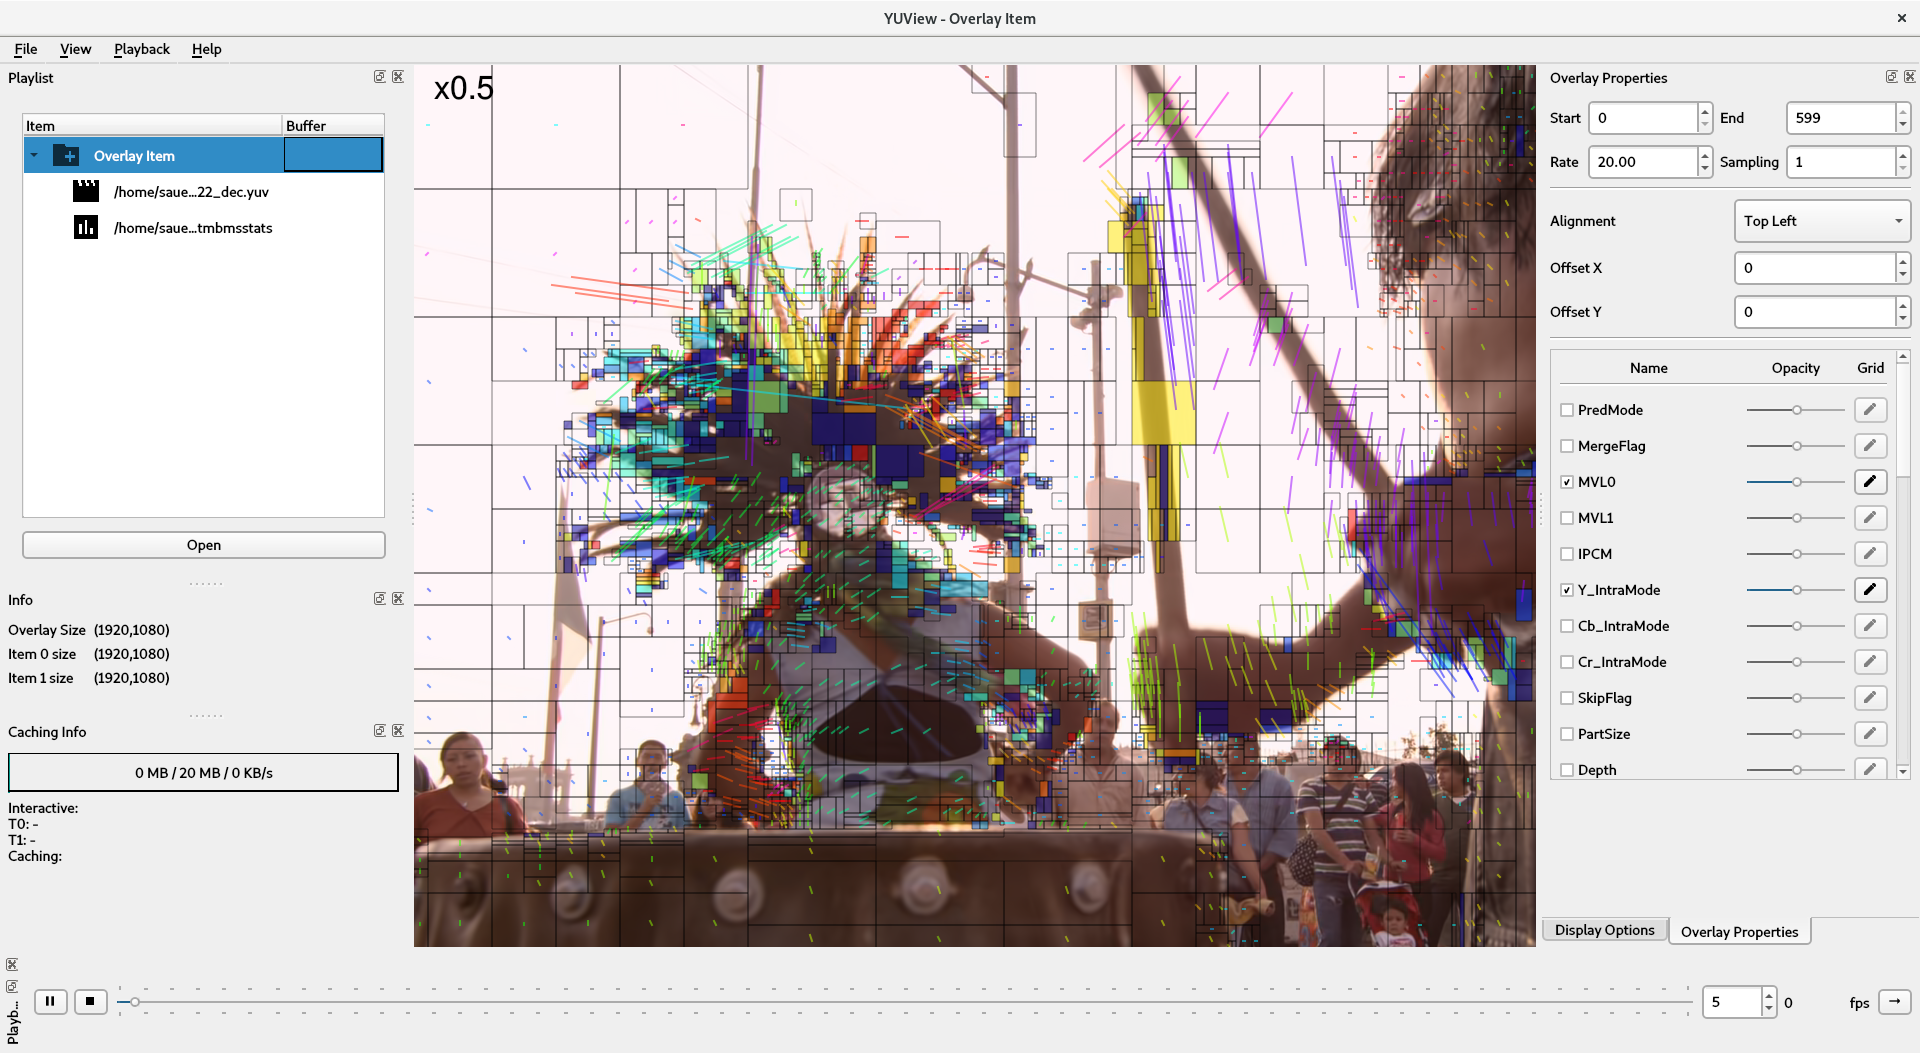
\includegraphics[width=0.8\linewidth]{figures/YUView}
  \caption{YUView}
  \label{fig:yuview}
\end{figure}

\begin{figure}[htpb]
  \centering
  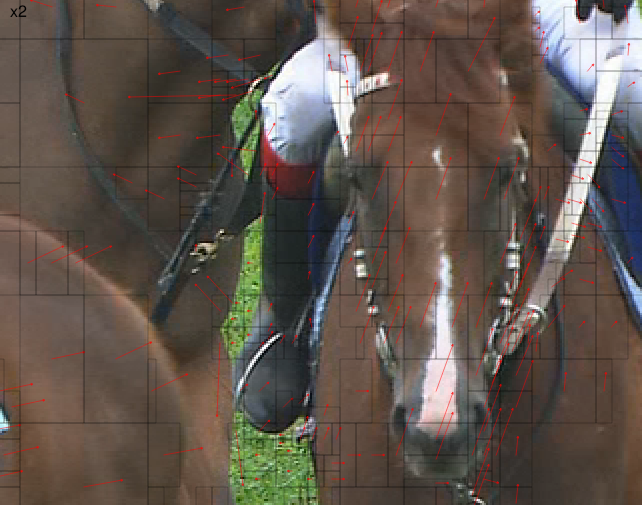
\includegraphics[width=0.5\linewidth]{figures/raceHorsesShot2MotionVectors}
  \caption{Motion vectors}
  \label{fig:motion-vectors}
\end{figure}


\begin{figure}[htpb]
  \centering
  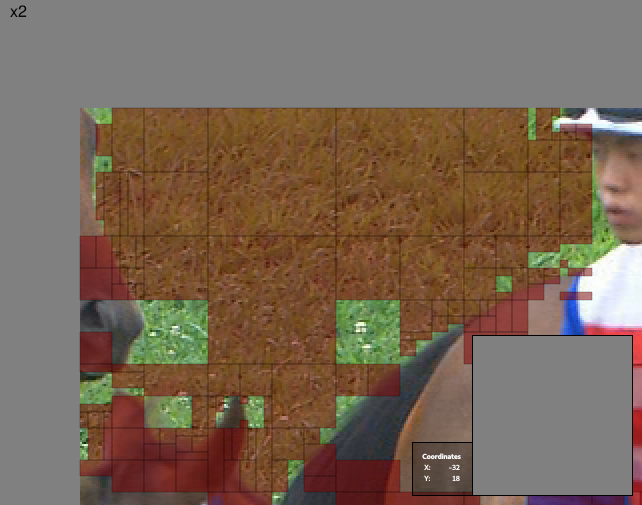
\includegraphics[width=0.5\linewidth]{figures/raceHorsesShot3SkipFlag}
  \caption{Skip flag}
  \label{fig:skip-flag}
\end{figure}

\subsection{Adding statistics}
\label{sec:adding-statistics}

In order to add further block statistics, do the following:


\begin{description}
\item[source/Lib/CommonLib/dtrace_blockstatistics.h]
  Add your statistic to the BlockStatistic enum:	
\begin{minted}{c++}
enum class BlockStatistic {
  // general
  PredMode,
  PartSize,
  Depth,
\end{minted}
  
Further, add your statistic to the map blockstatistic2description:
\begin{minted}{c++}
static const std::map<BlockStatistic, 
  std::tuple<std::string, BlockStatisticType, std::string>> 
  blockstatistic2description =
{
  { BlockStatistic::PredMode, 
    std::tuple<std::string, BlockStatisticType, std::string>
    {"PredMode", BlockStatisticType::Flag, ""}},
  { BlockStatistic::MergeFlag,
    std::tuple<std::string, BlockStatisticType, std::string>
    {"MergeFlag", BlockStatisticType::Flag, ""}},
  { BlockStatistic::MVL0,
    std::tuple<std::string, BlockStatisticType, std::string>
    {"MVL0", BlockStatisticType::Vector, "Scale: 4"}},
  YOURS
\end{minted}


\item[source/Lib/CommonLib/dtrace_blockstatistics.cpp] All code for
  writing syntax elements is kept in this file in
  getAndStoreBlockStatistics. This function is called once for each
  CTU, after it has been en/decoded. The following macros have been
  defined to facilitate writing of block statistics:
\begin{minted}{c++}
DTRACE_BLOCK_SCALAR(ctx,channel,cs_cu_pu,stat_type,val)   
DTRACE_BLOCK_SCALAR_CHROMA(ctx,channel,cs_cu_pu,stat_type,val)
DTRACE_BLOCK_VECTOR(ctx,channel,cu_pu,stat_type,v_x,v_y)    
DTRACE_BLOCK_AFFINETF(ctx,channel,pu,stat_type,v_x0,v_y0,v_x1,v_y1,v_x2,v_y2) 
\end{minted}

An example:
\begin{minted}{c++}
DTRACE_BLOCK_SCALAR(g_trace_ctx, D_BLOCK_STATISTICS_ALL, 
  cu, GetBlockStatisticName(BlockStatistic::PredMode), cu.predMode);
\end{minted}


\item[Block statistics for debugging] The statistics can also be used
  to write out other data, not just syntax elements. Add your
  statistics to dtrace_blockstatistics.h. Where it should be used the
  following headers have to be included:
\begin{minted}{c++}
#include "dtrace_next.h"
#include "dtrace_blockstatistics.h"
\end{minted}
\end{description}





\section{Using the stream merge tool}
\label{sec:stream-merge-tool}

The StreamMergeApp tool takes multiple single-layer (singe nuh_layer_id) bistreams 
as inputs and merge them into a multi-layer bistream by interleaving the NALUs 
from the input single layer bistreams. During the merge, the tool assigns a new unique
nuh_layer_id for each input bitstream. Then the decoder could specify which layer 
bitstream to be decoded through the command line option "-p nuh_layer_id". 

\subsection{Usage}
\label{sec:stream-merge-usage}

\begin{minted}{bash}
StreamMergeApp 	<bitstream1> <bitstream2> [<bitstream3> ...] <outfile>
\end{minted}

The command line options bistreamX specify the file names of the input single-layer 
bistreams. At least two input bitstreams need to be specified. The merged multi-layer 
bistream will be stored into the outfile.

\end{document}
